\chapter{Étude numérique}
\label{Chap::Simu::Analysis}
	\minitoc

	Après avoir évoqué diverses propriétés des amas globulaires de notre galaxie puis étudié certains résultats
	analytiques concernant les propriétés dynamiques des systèmes auto-gravitant, il est temps de mener des
	expériences numériques. Nous présenterons dans un premier temps le code d'évolution dynamique que nous avons
	utilisé, les conditions initiales de nos expériences et enfin les différentes observables de nos simulations.

	% \todo[inline]{FAIRE LA TRANSITION EN ANNONÇANT POURQUOI ON PASSE D'UNE DESCRIPTION FLUIDE À UNE PARTICULE À NOUVEAU.}

	% Après avoir mentionné l'importance des collisions à plusieurs corps pour expliquer le vieillissement des amas
	% d'étoiles, nous sommes passés dans la limite fluide afin de voir si d'autres phénomènes pouvait participer à
	% cette évolution. Nous allons maintenant nous tourner vers les simulations numériques.
	% Nous commencerons par présenter le treecode public Gadget-2. Nous enchaînerons sur la génération de nos
	% conditions initiales. Nous terminerons sur la présentation des diagnostiques nous servant à analyser les
	% simulations.

	% Après avoir montré l'importance des collisions à plusieurs corps dans les amas, puis être passé dans la
	% limite fluide afin de voir si d'autres phénomènes pouvait aussi faire évoluer ces amas. Nous nous retrouvons à
	% nouveau avec un système de particules que nous allons faire évoluer. Attention, il ne s'agit pas d'étoiles mais
	% de macro particules ayant une masse et une taille bien supérieur à celles des étoiles composant normalement ces
	% objets.

	% Les problèmes à $N$ corps sont des problèmes physiques extrêmement complexes mathématiquement: ils
	% font partie d'une famille d'équation du second ordre qui n'ont pas de solution pouvant
	% s'exprimer avec les fonctions mathématiques usuelles. Le seul cas connu pouvant s'écrire
	% simplement est le problème à 2 corps.

	\section{Le programme de simulation}
		% \todo[inline]{Parler macro-particule et limite fluide pour le $N$-corps.}

		Les expériences numériques que nous souhaitons réaliser ont pour objectif de modéliser l'évolution
		dynamique d'un système auto-gravitant. Dans ces simulations, nous souhaitons respecter au mieux le
		système dans son approche macroscopique (correspondant à la limite fluide de nos simulations) tout en
		laissant la possibilité à certains effets microscopiques d'apparaître (accrétion, relaxation).

		% Notre objectif est de résoudre numérique les équations de Vlasov-Poisson. Pour ceci, nous utilisons la
		% traditionnelle méthode $N$-corps: la fonction de distribution est échantillonée par des particules de
		% taille $\epsilon$, afin d'adoucir la force à petite échelle. En effet, nous souhaitons être au plus
		% proche de la limite fluide pour éviter les effets de relaxation à $N$-corps.

		% Le programme que nous utilisons pour faire évoluer notre système est
		Dans ce contexte, le programme que nous utilisons pour faire évoluer notre système est
		\textsc{Gadget-2}~\footnote{\url{http://www.mpa-garching.mpg.de/gadget/}} (voir \cite{gadget2} et \cite{gadget1}),
		écrit par Volker \textsc{Springel}.
		Ce programme allie un octree pour la gestion spatiale des particules et un algorithme de type \og
		prédicteur-correteur\fg pour la partie temporelle.
		% Ce programme allie un octree pour calculer le potentiel avec un schéma d'intégration temporel de type \og prédicteur
		% correcteur\fg d'ordre 2 basé sur un \og leag-frog\fg.

		% En plus de permettre de faire des simulations cosmologiques, gadget implémente la physique nécessaire
		% pour faire des simulations de galaxie avec du gaz. Ou juste des simulations de systèmes de particules
		% sans effets autre que l'attraction gravitationnelle.

		% Ainsi, seule une petite partie de ce qu'il fait nous intéresse. En effet, nous n'allons utiliser que les options
		% concernant l'oct-tree. Toutes les autres options ne concernent que les simulations
		% cosmologiques ou pourraient induire un comportement non voulu du système ou du programme.
		% qui nous ferait perdre de la précision sur
		% les calculs.

		\subsection{Calcul du potentiel: $\mathrm{k}^\mathrm{d}$-Tree}
			\label{Sec::KdTree}
			% Numériquement, les problèmes à $N$-corps sont très couteux en terme de calculs. En effet, un
			% calcul simple de la force s'appliquant sur une particule peut se faire en sommant la force exercée par
			% chacune des autres particules dessus. Cette méthode nécessite une première itération sur toutes les
			% particules de la simulation, qui sera ensuite répétée pour toutes les particules. Elles
			% nécessitent donc $N^2$ opérations.
			% Ainsi, dés que nous allons tenter de simuler un grand nombre de particules, sur un grand nombre
			% de temps dynamique, les temps de calculs vont exploser.
			% Nous avons donc besoin d'un algorithme qui va nous permettre de faire évoluer le
			% système avec beaucoup de particule et sur un grand nombre de temps dynamique, dans des temps
			% raisonnables.

			Un calcul direct des forces d'interaction entre chaque particules nécessite $N^2$ opérations.
			Bien que très couteuse, cette méthode est encore très utilisée pour suivre finement la dynamique
			d'un amas. À ce jour, la plus grosse simulation $N$-corps est le travail de D. Heggie avec
			presque 300 000 particules (voir sa présentation au trimestre Gravasco) en utilisant la version
			GPU de NBODY6. Dans la limite fluide, nous aurons parfois besoin d'un grand nombre de particules
			pour représenter la fonction de distribution dans l'espace des phases. Nous avons donc besoin
			d'une approche nous permettant d'accélérer les calculs. Il existe de nombreuses méthodes pour
			ceci (une revue des différentes méthodes a été faîte dans \citet{2014arXiv1404.5175C}). Celle
			que nous utilisons est basée sur un algorithme en arbre.

			% Un tel algorithme a été développé par J. Barnes et P. Hut dans~\citet{1986Natur.324..446B}. Il se
			% base sur un kd-tree de dimension 3, un oct-tree. Le principe est de subdiviser l'espace,
			% représenté par un cube, en 8 sous cubes, eux-mêmes subdivisé en 8 nouveaux sous cubes...
			% Chaque cube est à nouveau divisé s'il contient encore trop de particules.
			% Dans~\citet{1986Natur.324..446B}, ils arrêtent de subdiviser un cube quand il ne contient plus
			% qu'une particule; en pratique nous nous arrêterons lorsqu'un cube contiendra une quinzaine de
			% particules. La figure~\ref{Fig::KDTree::Repr} montre la structure d'un quad-tree, un
			% kd-tree à 2 dimension se construisant de la même façon.

			Un tel algorithme a été appliqué en astrophysique pour la première fois par
			\cite{1986Natur.324..446B}. Il se base sur une représentation en arbre
			($\mathrm{k}^\mathrm{d}$-Tree) des particules du système de dimension 3, cet arbre est appelé
			octree ($k=2$, $d=3$). Le principe est de subdiviser un espace cubique en 8 sous cubes, eux-mêmes subdivisés en
			8 nouveaux sous cubes... Chaque cube est à nouveau divisé s'il contient encore trop de
			particules.
			% Les auteurs arrêtent de diviser un cube
			% quand il ne contient plus qu'une particule;
			En pratique nous nous arrêterons lorsqu'un cube contiendra au plus $N_\mathrm{max}=15$ particules.
			Les carrées et les points de la figure~\ref{Fig::KDTree::Parcours} montre la structure d'un
			quadtree ($k=2$, $d=2$) se construisant de la même façon.
			% La figure~\ref{Fig::KDTree::Parcours} montre la structure d'un quadtree (un kd-tree à 2
			% dimension) se construisant de la même façon.

			Avant de continuer il peut être utile de définir un peu de vocabulaire lié aux arbres:
			\begin{itemize}
				\item la racine constitue la base de l'arbre;
				\item un nœud est un cube ayant un père et des fils, il s'agit d'un embranchement;
				\item une feuille est un cube n'ayant plus de fils, et donc terminant une branche de
					l'arbre;
				\item une branche est le chemin à suivre pour aller de la racine vers une feuille.
			\end{itemize}

			% \begin{figure}
				% \begin{center}
					% 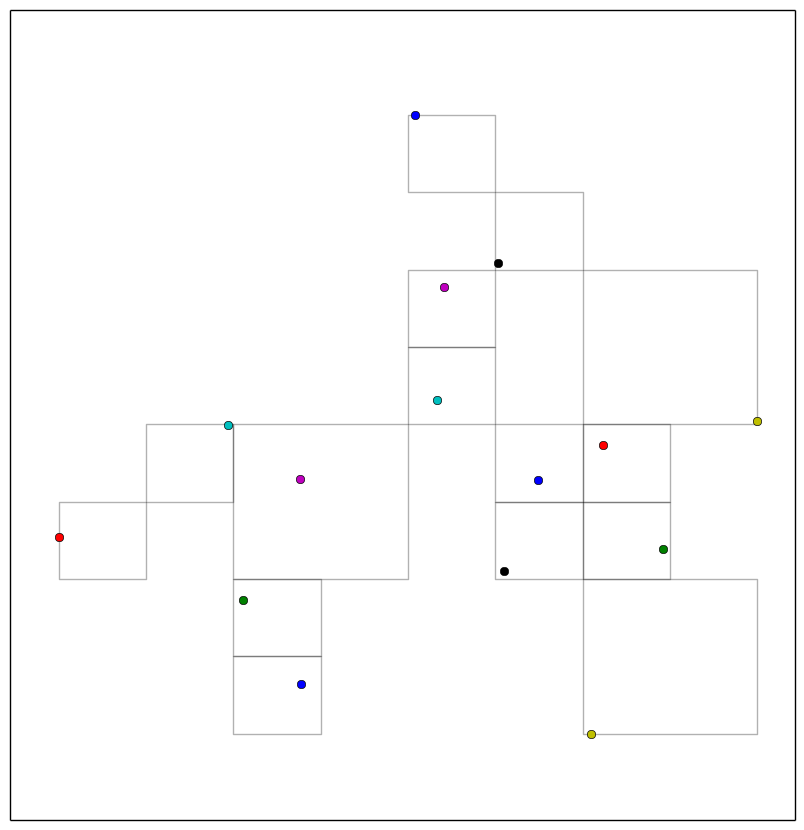
\includegraphics[scale=0.4]{repre_tree}
					% \caption{\label{Fig::KDTree::Repr}Représentation de la structure d'un quad-tree
						% (kd-tree en 2 dimension) sur 15 particules.}
				% \end{center}
			% \end{figure}

			Une fois l'arbre construit, le calcul de la force ou du potentiel se fait en descendant dans les nœuds
			tant que l'angle d'ouverture reste supérieur à une valeur critique.
			% (les cubes qui ont été subdivisés) selon un critère: l'angle d'ouverture du cube par rapport à une
			% particule est-il supérieur à une valeur $\theta$ choisie.
			L'angle d'ouverture correspond à la taille angulaire du nœud vue par la particule sélectionnée.
			Si cette taille est suffisamment petite, nous n'entrons pas à l'intérieur et résumons son
			contenu à une macro-particule, sinon la descente continue (voir figure~\ref{Fig::KDTree::Parcours})% nous testons chacune des
			% subdivisions. Par exemple, sur la figure~\ref{Fig::KDTree::Parcours}, le cône vert indique un
			% cube que nous ne voulons pas parcourir, tandis que le rouge nous indique qu'il faut continuer
			% à descendre.

			\begin{figure}
				\begin{center}
					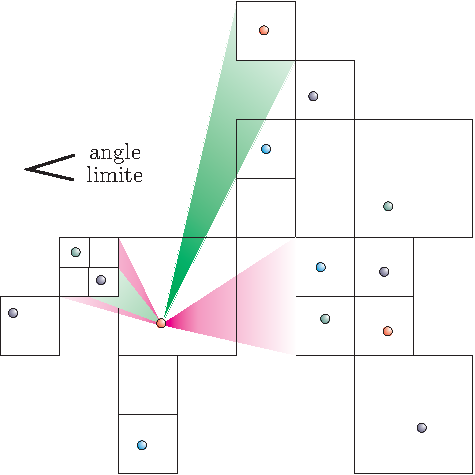
\includegraphics[scale=1.0]{accept_treev2}
					\caption{\label{Fig::KDTree::Parcours}Représentation du critère sur l'angle
					d'ouverture pour ouvrir ou non un cube. Le cône vert indique un cube qu'il
					n'est pas nécessaire d'ouvrir, le cône rouge indique un cube à ouvrir.}
				\end{center}
			\end{figure}

		\subsection{Lissage de la force}

			%Nous souhaitons nous placer dans la limite fluide afin
			%de minimiser les effets de relaxations dû aux
			%collisions à deux corps. Pour cela, nous pouvons jouer
			%sur deux paramètres : le nombre de particules que nous
			%mettons dans le système, et le paramètre de lissage.
			%Étant limité en temps, nous ne pouvons pas lancer de
			%simulations avec un très grand nombre de corps : les
			%plus grosses simulations que nous lançons ont 100 000
			%particules, et occasionnellement 500 000. Pour une
			%évolution pendant 100 temps dynamiques, elles prennent
			%environ 709 minutes en les faisant tourner sur 8 cœurs,
			%et cela peut aller jusqu'à 1020 minutes.

			%Toute la théorie a été faîte dans le cadre de l'équation de vlasov, et donc en supposant que nos
			%objet se comporte comme des fluides. Nous devons donc être sûr que les collisions interne de nos
			%objet n'aient que peu d'influence.
			%Pour éviter les soucis de divergence de la force lorsque deux
			%particules deviennent très proches, un paramètre de lissage (softening) a été introduite de façon à ce
			%que la force ne dépasse pas une valeur minimale. C'est aussi

			% Toute la théorie ayant été faite dans le cadre de la limite fluide, % l'équation de Vlasov,
			% nous souhaitons nous y placer aussi % dans la limite fluide
			% afin de nous approcher du mieux possible des conditions théoriques, mais
			% aussi pour minimiser les effets de relaxations à deux corps qui ne manqueront pas d'intervenir sur le long terme
			% dans cette description de nos système. Pour cela, nous allons jouer sur
			% le paramètre de lissage de la force qui adoucit cette dernière. Ceci ce traduit par le potentiel
			% effectif suivant:
			Toute la théorie ayant été faite dans le cadre de la limite fluide, % l'équation de Vlasov,
			il est important de l'approcher du mieux possible. %nous souhaitons nous y placer aussi % dans la limite fluide
			% afin de nous approcher du mieux possible des conditions théoriques, mais
			Les effets de relaxations à deux corps sont également susceptibles d'intervenir sur le long
			terme, il nous faut pouvoir les faire intervenir. % dans cette description de nos système.
			Pour cela, nous allons jouer sur
			le paramètre de lissage de la force $\epsilon$ dans le potentiel
			effectif suivant:
			\todo[inline]{Je ne met pas la formule de Springel par ce que je ne la comprend pas vraiment. Il
			utilise la convolution d'un dirac représentant la particule avec un "spline-kernel". Par
			contre, pour la définition du $\epsilon$, c'est censé être équivalent à ceci.}
			% Classiquement, ce paramètre de lissage
			% est une borne, en distance, en deçà de laquelle nous considérons un potentiel minimum pouvant
			% s'écrire sous la forme:
			\begin{align}
				% \psi(r_{ij} \sim 0) = - G \dfrac{m_i}{r_{ij} + \epsilon}
				% \psi(r_{i}) = - G \sum_{j \neq i}^{N}\dfrac{m_i}{|r_{i}-r_j| + \epsilon}
				\psi(r_{i}) = - G \sum_{j \neq i}^{N}\dfrac{m_i}{r_{ij} + \epsilon}
			\end{align}
			où $r_{ij}$ est le module de distance entre les particules $i$ et $j$
			Afin que la limite fluide soit suffisamment bien décrite, nous devons choisir ce
			paramètre tel que d'une part la sphère de rayon $\epsilon$ contienne un nombre $N_\epsilon$ suffisant de particules
			mais que d'autre part $N_\epsilon$ soit suffisamment petit devant le nombre total de particules du système.
			Ce nombre $N_\epsilon$ peut s'évaluer de la façon suivante; considérons le paramètre
			\begin{align*}
				\alpha = \dfrac{\rho_\epsilon}{\rho_\mathrm{moy}}
			\end{align*}
			où $\rho_\epsilon$ la densité d'un volume de rayon $\epsilon$ suffisamment petit pour être
			supposé homogéne et $\rho_\mathrm{moy}$ la densité
			moyenne de l'objet. Toutes les particules ayant la même masse, nous pouvons écrire:
			\begin{align}
				N_\epsilon    = \alpha N \(\dfrac{\epsilon}{R} \)^{3}
			\end{align}
			$N$ étant le nombre total de particules de l'amas. Les paramètres $N$, $R$ et $\alpha$ étant fixés, nous sommes
			ainsi libres de choisir $N_\epsilon$ ou $\epsilon$ pour répondre à nos besoins.
			% \begin{align}
				% \alpha = \dfrac{\rho_\epsilon}{\rho_\mathrm{moy}} = \dfrac{\rho_\epsilon}{M} \frac{4}{3} \pi R^3
			% \end{align}
			% où $M$ est la masse totale de l'amas, $R$ le rayon de l'amas, et $\rho(0)$ la densité centrale de
			% l'amas. La densité d'un volume de taille $\epsilon$ en fonction de la densité moyenne de l'amas
			% s'écrit alors:
			% \begin{align}
				% \rho_\epsilon &= \alpha \rho_\mathrm{moy}	\notag \\
				% \intertext{le nombre de particule dans un volume de rayon $\epsilon$ s'écrit:}
				% N_\epsilon    &= \alpha \frac{4}{3} \pi \epsilon^3 \dfrac{3N}{4\pi R^3}	\notag \\
					      % &= \alpha N \( \dfrac{\epsilon}{R} \)^{3}
			% \end{align}
			% $N$ étant le nombre total de particules de l'amas. $N$, $R$ et $\alpha$ étant fixés, nous sommes
			% ainsi libres de choisir $N_\epsilon$ ou $\epsilon$ pour répondre à nos besoins.

		\subsection{\og Leap-frog\fg et pas de temps}

			Gadget-2 utilise un schéma d'intégration temporelle de type  \og prédicteur-correcteur\fg qui se
			ramène à un leap-frog dont nous allons étudier le fonctionnement.

			% Le problème simulé peut s'écrire ainsi:
			Pour chaque particule de masse $m$ dy système, le problème à résoudre s'écrit:
			\begin{align*}
				\begin{cases}
					\dfrac{\vdr}{\dx{t}} = \vec{v} \\
					\\
					m\dfrac{\vdx{\vec{v}}}{\dx{t}} = \vec{f}(\vec{r})
				\end{cases}
			\end{align*}
			il peut être approché par:
			\begin{align*}
				\begin{cases}
					\dfrac{\vec{r}_\mathrm{new} - \vec{r}_\mathrm{old}}{\Delta t} = \vec{v}_\mathrm{new} \\
					\\
					m\dfrac{\vec{v}_\mathrm{new} - \vec{v}_\mathrm{old}}{\Delta t} = \vec{f}(\vec{r}_\mathrm{old}) = \vec{a}m
				\end{cases}
			\end{align*}
			La particularité du schéma est le décalage entre l'évaluation des positions est des vitesses:
			les positions vont être évaluées tous les $n\Delta t$ tandis que les vitesses vont l'être tout
			les $(n+\frac{1}{2})\Delta t$.

			Le schéma d'intégration s'écrit alors:
			\begin{align*}
				\begin{cases}
					\vec{v}_{n+1/2} = \vec{v}_{n-1/2} + \Delta t\vec{f}(\vec{r}_n) \\
					\\
					\vec{r}_{n+1} = \vec{r}_n +\Delta t\vec{v}_{n+1/2}
				\end{cases}
			\end{align*}

			Le code Gadget-2 opére une gestion fine du pas de temps $\Delta t$ de manière à ce que le calcul
			de:
			\begin{align*}
				\Delta t = \sqrt{\dfrac{2\eta\epsilon}{|\vec{a}|}}
			\end{align*}
			reste dans un intervalle de contrôle.
			Le paramètre $\eta$ permet de contrôler la précision de l'intégration.
			% Il reste à déterminer comment le pas de temps $\Delta t$ est calculé dans Gadget-2. La première chose à
			% laquelle faire attention est que chaque particules a son propre pas de temps. Ce pas de temps
			% va évoluer au cours de la simulation, tout en restant bornée par un pas de temps minimum et un
			% pas de temps maximum. Le pas de temps est donné par la formule:
			% \begin{align*}
				% \Delta t = \sqrt{\dfrac{2\eta\epsilon}{|\vec{a}|}}
			% \end{align*}
			% où $\epsilon$ est le paramètre de lissage de la force, $|\vec{a}|$ le module de l'accélération
			% de la particule et $\eta$ un paramètre permettant de contrôler la précision de l'intégration.

		%\subsection{Unités}

			%Dans ce fichier, nous n'allons jouer que sur certains paramètres :
			%\begin{itemize}
				%\item \verb|OmegaLambda| : paramètre cosmologique représentant la densité d'énergie du
					%vide, en le mettant à 0, nous faisons savoir à \textsc{Gadget-2} que nous ne faisons pas
					%de simulation cosmologique.
				%\item \verb|UnitLength_in_cm|, \verb|UnitMass_in_g| et \verb|UnitVelocity_in_cm_per_s|
					%sont les unités dans lesquelles sont données, respectivement, les positions, masses et vitesses des particules en
					%centimètre, gramme en centimètre par seconde. Ce sont ces facteurs de conversion
					%qui donne l'unité de temps interne à \textsc{Gadget-2}. Nous utilisons
					%les parsecs ($ 1 pc = 3.086 \times 10^{18} cm$) pour les positions, les kilogrammes
					%($1 kg = 1000 g$) pour la masse, et les mètres par seconde ($ 1 m.s^{-1} = 10^2 cm.s^{-1}$)
					%pour les vitesses. Ces unités nous donnent comme unité de temps
					%interne :
					%\begin{align}
						%v &= \frac{d}{t} \notag \\
						%t &= \frac{d}{v} \notag \\
						%t &= \frac{3.086 \times 10^{18}}{10^2} = 3.086 \times 10^{16} s \notag \\
						%t &= 9.77894 \times 10^8 ans
					%\end{align}
				%\item \verb|SofteningStarsMaxPhys| : paramètre de lissage de la force, permettant d'éviter
					%qu'elle \og~n'explose~\fg~à cause d'une collision entre 2 particules trop proches.
					%C'est sur ce paramètre qu'il faut jouer pour assurer la stabilité du système sur
					%un grand nombre de temps dynamiques.
				%\item \verb|ErrTolTheta| : représente l'angle d'ouverture, ou résolution angulaire, minimum.
					%Celui-ci est fixé à $0.5$ et n'est plus modifié ensuite.
			%\end{itemize}






		%Pour fonctionner, \textsc{Gadget-2} a besoin d'un fichier de
		%configuration, dans lequel nous devrons jouer sur certains
		%paramètres, et d'un fichier de conditions initiales respectant
		%un format précis.

		%\subsection{Pas de temps}
		%\subsection{Paramètre de l'arbre}
		%\subsection{Format de sortie}

		%\subsection{Fichier de conditions initiales}

			%Le fichier de conditions initiales doit avoir le format suivant :
			%\begin{enumerate}
				%\item un en-tête contenant le nombre de particule de chaque type (~Gaz, Halo, Disque, Bulbe, Étoiles, Bndry~),
				%la masse pour chaque type, divers autres informations utiles essentiellement aux simulations cosmologiques,
				%\item les positions de chaque particules,
				%\item leurs vitesses,
				%\item un identifiant permettant de repérer chaque particule.
			%\end{enumerate}
			%Chaque bloc devant être encadré par sa taille en mémoire.

		%\subsection{Fichier de configuration}



	\section{Conditions initiales}

		% Pour générer des nombres aléatoires dans l'intervalle voulu, nous utiliserons une
		% implémentation de la fonction \verb|ran2| tiré de~\citet{NumericalRecipesC}.

		Pour mener à bien nos expériences numériques, nous avons besoin de configurations: une sphère de King,
		une sphère de Hénon et un bain thermique.

		\subsection{Le modèle de \textsc{King}}

			Les particules du modèle de King, de paramètres $W_0$, $\sigma$ et $r_c$ sont générées en
			utilisant une méthode d'acceptation-rejection que nous allons décrire. À partir de ces 3
			paramètres, nous pouvons résoudre l'équation de poisson~\ref{King-Pois} donnant le potentiel
			pour le modèle de King. Nous pouvons alors calculer le potentiel central $\psi(0)$ et l'énergie
			de libération $E_l$.
			% Ces particules sont telles que $r<R$ et $v<v_\mathrm{max}$, avec $R$ et $v_\mathrm{max}$ défini tels que:
			Toutes les particules de la sphère de King ont une vitesse dont le module de vitesse est
			inférieur à une vitesse $v_\mathrm{max}$ et leurs distance au centre est inférieur à un rayon
			$R$. Ces bornes sont définies tel que:
			% Pour obtenir nos conditions initiales, qui devront suivre un profil de \textsc{King}, nous
			% allons utiliser la méthode de réjection. Nous allons tirer aléatoirement la position et la
			% vitesse des particules dans une boîte, puis nous n'en garderons qu'une partie en utilisant la
			% fonction de distribution dans l'espace des phases comme une densité de probabilité. Pour
			% commencer, nous utilisons les limites du modèle pour restreindre nos tirages à une boîte de
			% taille \mbox{$\left[ - R; R \right]$} pour les distances et \mbox{$\left[ -v_{\mathrm{max}};
			% v_{\mathrm{max}}\right]$} pour les vitesses, avec:
			\begin{itemize}
				\item $v_{\mathrm{max}}$ la vitesse maximum: %l'énergie totale du système est bornée supérieurement par l'énergie de libération :
					\begin{align}
						% E = \dfrac{1}{2} m v_i^2 + m\psi(r) &< E_l \notag \\
						% E_l - m\psi(r) &> \dfrac{1}{2} m v_i^2 \notag \\
						% v_\mathrm{max}^2 = 2\(\dfrac{E_l}{m} - \psi(r)\) &> v_i^2 \notag \\
						v_{\mathrm{max}} = \sqrt{2\(\dfrac{E_l}{m} - \psi(0)\)}% > v_i &> - \sqrt{2\(\dfrac{E_l}{m} - \psi(0)\)} = - v_{\mathrm{max}}
					\end{align}
				\item $R$ le rayon de la sphère: ce rayon est obtenue en résolvant numériquement
				% \item $R$ la distance maximum : cette distance est obtenue pour
					% $m\psi(R) = E_l$.
					$\rho(R) = 0$
			\end{itemize}
			% où $E_l$, l'énergie de libération est déterminé, grâce au théorème de Gauss, par:
			% \begin{align*}
				% \dfrac{E_l}{m} = -\dfrac{GM}{R}
			% \end{align*}

			Les paramètres $R$ et $v_\mathrm{max}$ étant connus, nous tirons aléatoirement les positions
			$x_i$, $y_i$, $z_i$ telles que $|\vec{r}_i| \leq R$; puis les vitesses $v^x_i$, $v^y_i$, $v^z_i$
			telles que $|\vec{v}_i|\leq v_\mathrm{max}$.
			% Formule obtenue en considérant que l'énergie qu'une particule de vitesse nulle au centre du
			% système doit acquérir est donnée par l'énergie su
			% Il nous faut donc connaître le potentiel, qui est obtenu numériquement.

			%Le potentiel n'ayant pas d'expression analytique, nous
			%allons devoir réutiliser notre algorithme de résolution numérique utilisé dans les chapitres
			%précédents pour modèliser un King.

			%Il nous faut aussi pouvoir redimensionner les quantités obtenues. Pour cela, le
			%programme récupère dans un fichier de configuration les dispersions de vitesse
			%$\sigma_v^2$, rayon de c\oe ur $r_c$, temps de relaxation $T_c$ et distance au
			%soleil $R_\odot$ dans les unités du catalogue de \textsc{Harris}. Toutes sont
			%ensuite transformées en unités SI (~mètre, kilogramme, seconde~). Comme nous
			%avons pu le voir dans le chapitre~\ref{King::Chapitre} traitant du modèle de
			%King, la masse $m$ d'une particule n'influence pas le profil de densité final :

			% Les simulations utilisant le modèle de \textsc{King} s'effectueront en unités physique,
			% En connaissant le rayon de cœur $r_c$ et la dispersion de vitesse $\sigma_v$, il est possible de
			% déduire la dernière quantité nécessaire au dimensionnement: $\rho_0$ (défini dans le
			% chapitre~\ref{King::Chapitre}). Reste ensuite une degré de
			% liberté qui nous permet de choisir entre la masse d'une particule ou le nombre de
			% particules du système.
			% \begin{align}
				% r_c^2 &= \dfrac{\sigma^2}{4\pi G m \rho_0} \notag \\
				      % &= \dfrac{(\sigma_v^2)^2 m}{8\pi G m \rho_0} \notag \\
				      % % &= \dfrac{(\sigma_v^2)^2}{8\pi G \rho_0} \notag \\
				% \Rightarrow \rho_0 &= \dfrac{(\sigma_v^2)^2}{8\pi G r_c^2}
			% \end{align}
			% Pour redimensionner la densité, nous n'avons donc pas besoin de connaître la
			% masse d'une particule. Ce constat nous permet de laisser ce paramètre libre et
			% de jouer sur le nombre de particules dans le système. En effet, une fois la
			% densité obtenue, nous pouvons l'intégrer sur le volume de l'amas pour trouver la
			% masse totale de ce dernier, puis, connaissant le nombre de particules, en déduire
			% la masse d'une étoile par la relation :
			% \begin{align}
				% m = \dfrac{M_{tot}}{\text{Nombre de particules}}
			% \end{align}
			% Déduire le reste des paramètres utiles pour le redimensionnement est ensuite
			% assez simple.
			% La distance maximum $r_{\mathrm{max}}$ est déduite de la résolution
			% numérique des équations.

			% Pour pouvoir tout redimensionner, nous avons aussi besoin de connaître l'énergie
			% de libération de l'amas $E_l$. Pour cela, nous utilisons le théorème de \textsc{Gauss}.
			%et un petit raisonnement simple.
			% Par définition, nous avons :
			% \todo[inline]{Reformuler cette partie sur les énergies, je ne pense pas transmettre la bonne
			% idée.}
			% \begin{align}
				% E_\mathrm{min} < E < E_l < 0 \ &\text{ et } \ E_l = \frac{p^2}{2 m} + m \psi(r)
				% \intertext{soit:}
				% \intertext{le maximum du potentiel est atteint lorsque $p=0$, en appliquant le théorème
				% de Gauss au bord du système:}
				% \psi(r) = \frac{1}{m}\(E_l - \frac{p^2}{2 m}\)
				% \intertext{La valeur maximale du potentiel est donc atteinte pour $p = 0$ :}
				% \psi_\mathrm{max} = \psi(R) = \frac{E_l}{m} \stackrel{\mathrm{Gauss}}{=} -\frac{G M}{R}
				% \intertext{Hors du système, le théorème de \textsc{Gauss} nous dit qu'il peut être vu comme une particule ponctuelle de masse $M$. Le potentiel hors de l'amas s'écrit donc :}
				% \psi(r) = -\frac{G M}{r}
				% \intertext{Par continuité, nous avons :}
				% \psi(R) = \frac{E_l}{m} = -\frac{G M}{R}
			% \end{align}

			% Pour générer des nombres aléatoires dans l'intervalle voulu, nous utilisons la
			% fonction \verb|double ran2(long seed)| tiré de~\citet{NumericalRecipesC}, dont
			% nous nous servont ainsi :
			% \lstset{language=C, label=algo::tirage, frame=shadowbox}
			% \begin{lstlisting}
				% double  x  = rmax - 2.0 * rmax * ran2(seed),
					% y  = rmax - 2.0 * rmax * ran2(seed),
					% z  = rmax - 2.0 * rmax * ran2(seed),
					% vx = vmax - 2.0 * vmax * ran2(seed),
					% vy = vmax - 2.0 * vmax * ran2(seed),
					% vz = vmax - 2.0 * vmax * ran2(seed);
			% \end{lstlisting}

			% Jusqu'ici, nous avons généré nos particules dans un cube. L'étape suivante consiste à les
			% filtrer selon leur distance au centre.
			% L'étape suivante consiste à les filtrer en utilisant la fonction de distribution dans l'espace
			% des phases comme une densité de probabilité.
			% Pour le modèle de King, nous connaissons $f(E)$ et non $f(\vec{r}, \vec{v})$; nous calculons
			% donc l'énergie à partir des positions et vitesses.

			Nous utilisons alors la fonction de distribution du modèle de King (voir la
			relation~\ref{King::Eq::DistribFunc}) normalisée à $1$ comme une densité de probabilité, en
			utilisant l'énergie $E_i = \frac{1}{2}mv_i^2 + m\psi(r_i)$, pour accepter ou rejeter la
			particule $i$ fabriquée. Le taux de rejection est de l'ordre de $99.99\%$
			mais la vitesse des ordinateurs permet d'utiliser cette méthode très simple pour fabriquer un
			modèle de King discret.
			% mais cette méthode permet de générer simplement un modèle de King.

			% À la fin, nous regardons la probabilité d'avoir une
			% particule avec ces valeurs de positions et vitesses et nous tirons un nombre aléatoire nous
			% disant si la particule est conservée ou non.


			% Notre système étant sphérique, nous ne devons pas avoir
			% de vitesse et de module de distance supérieurs,
			% respectivement, à $v_{\mathrm{max}}$ et
			% $r_{\mathrm{max}}$, de plus nous avons une probabilité
			% \mbox{$f(E)/f(E_\mathrm{min})$} d'avoir une particule
			% d'énergie $E$. Cette énergie minimale est l'énergie
			% potentielle d'une particule au centre de l'amas, et de
			% vitesse nulle. Une fois qu'une particule respecte ces
			% conditions et que \og les probabilités sont avec
			% elle\fg, nous l'enregistrons.

			% Le programme écrit au fur et à mesure les coordonnées cartésiennes et vitesses
			% des particules sélectionnées dans un fichier dans les unités standards : mètre
			% pour les distances et mètre par seconde pour les vitesses.

		\subsection{La sphère de Hénon}

			% Une sphère de Hénon est, comme son nom l'indique, une sphère de densité
			Nous appelons sphère de Hénon une sphère de densité
			constante possédant une distribution de vitesse suivant
			une loi de Gauss:
			\begin{align}
				f_H(r, v) = \rho_0 e^{-v^2/\sigma^2}
			\end{align}
			Nous générons donc indépendamment les positions selon une loi uniforme, et les vitesses selon
			une loi gaussienne. Le choix de la dispersion de vitesse $\sigma$ nous permet de choisir le rapport
			du Viriel $\gamma = -\dfrac{2E_c}{E_p}$.
			% La dernière étape consiste à modifier les vitesses pour mettre le système au
			% Viriel $\gamma = -\dfrac{2E_c}{E_p}$ voulu.

		\subsection{Bain thermique}

			Lors de notre étude numérique, nous allons avoir besoin de créer un objet nous permettant de
			simuler un bain thermique. Pour ceci, nous allons utiliser un cube homogène de côté $R_c$
			possédant un distribution de vitesse gaussienne de dispersion de vitesse $\sigma_c$.
			Nous jouerons sur ces deux paramètres pour tester l'influence du bain.

	\section{Observables des simulations}  %\label{Verif_gene}}

		% Maintenant que nous avons un générateur de conditions
		% initiales, il convient de le vérifier. C'est-à-dire d'utiliser
		% les coordonnées, vitesses et masses des particules pour
		% remonter à des quantités comme la densité ou l'énergie de
		% l'objet créé, puis de comparer ces quantités aux prédictions
		% théoriques. À des fins de Comparaison, nous avons généré un
		% profil de King avec \mbox{100 000} particules, qui se doit donc d'être
		% au Viriel, mais aussi d'avoir un profil de densité de type cœur-halo.

		Lors de nos expériences numériques, nous souhaitons étudier l'évolution des systèmes dans tout l'espace des
		phases. Nous avons donc construit un code effectuant le calcul de différentes observables spatiales
		(densité, position, rapport d'axes, etc) et cinétiques (énergies, température, etc).

		Toutes les courbes présentées dans cette section correspondent à un modèle de King de paramètre $W_0=6$, $r_c =
		3.5\mathrm{pc}$ et $\sigma_v = 2.9 \mathrm{km}.\mathrm{s}^{-1}$ généré avec 100 000 particules.

		% Nous en profiterons pour présenter toutes les quantités diagnostiqué.
		% densité, comme vu dans les précédents chapitres.

		% Pour faire les vérifications, nous avons choisi d'utiliser des histogrammes.

		\subsection{Recentrage}

			Pour calculer avec précision les différentes quantités physiques qui nous intéressent, il est
			important d'avoir la meilleure détermination possible du centre du système, qui a tendance à se
			déplacer. Ce déplacement peut se produire car la vitesse moyenne du système n'est pas exactement
			nulle, ou encore parce que des particules sont éjectées loin du système, emportant une partie
			notable de l'énergie.

			% Lors des simulations, nos systèmes peuvent se déplacer. Par exemple, un système isolé va voir sa
			% vitesse moyenne augmentée en perdant des particules. Ou encore parce que la vitesse moyenne du
			% système à $t=0$ n'est pas exactement nulle.

			Plusieurs méthodes sont envisageables pour recentrer le système. La première est de calculer le
			centre de gravité. Le problème posé par cette approche est que les particules très éloignées du
			centre système ont le même poids statistique que les particules située proche du centre.
			Le calcul du centre de gravité peut s'en trouver largement affecté.
			Par conséquent, nous devons calculer un centre donnant plus de poids aux
			particules se trouvant dans des zones denses du système. Il s'agit du \og centre de densité\fg,
			tel que décrit dans~\citet{1985ApJ...298...80C}. Le principe est de rechercher les $j$ plus
			proches voisins d'une particule et de regarder dans quel volume elles se répartissent; ceci nous
			donne la densité locale de la particule, et donc son poids selon la formule suivante:
			\begin{align}
				\rho_j^i = \dfrac{j-1}{V(r_j)}m
			\end{align}
			avec $j$ le nombre de voisin, $\rho_j^i$ la densité locale à la particule $i$, $V(r_j)$ le volume
			dans lequel se situent les $j$ voisins, et $m$ la masse d'une particule. Pour obtenir le centre
			de densité,
			nous faisons un calcul similaire au centre de gravité mais en pondérant chaque position par sa densité locale.

			Ce calcul peut s'avérer numériquement couteux, nous avons  donc adapté l'algorithme de l'octree
			pour accélérer le calcul.
			% Pour accélérer les calculs, nous utilisons la technique de l'octree décrite précédemment afin de chercher les $j$ plus
			% proches voisins, mais plutôt que d'utiliser l'angle d'ouverture, nous comparons
			% la distance entre la particule $i$ et le coin le plus proche de chaque cube à la distance entre
			% la particule $i$ et le voisin trouvé le plus lointain. Si le cube est plus proche, il est alors
			% sélectionné et nous testons ses fils ou les particules si nous sommes sur une feuille.

		\subsection{Masse et densité}

			\todo[inline]{En fait, j'ai les 2 versions: espacé logarithmiquement et "normal". J'en avais une
			3éme en chantier pour laquelle les bins était calculé de sorte que chacun aient le même nombre
			de particule, mais je ne l'ai jamais fini.}

			\begin{wrapfigure}{l}{0.40\textwidth}
				\begin{center}
					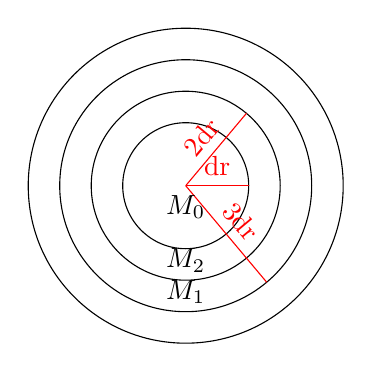
\begin{tikzpicture}[scale=0.8]
						\draw (2.5,2.5) circle(1);
						\draw (2.5,2.5) circle(1.5);
						\draw (2.5,2.5) circle(2);
						\draw (2.5,2.5) circle(2.5);
						\draw[red] (2.5,2.5) -- (3.5,2.5) node[midway, above] {$\mathrm{dr}$};
						\draw[red] (2.5,2.5) -- ++(50:1.5) node[sloped, above, midway] {$2 \mathrm{dr}$};
						\draw[red] (2.5,2.5) -- ++(-50:2) node[sloped, above, midway] {$3 \mathrm{dr}$};
						\draw (2.5,2.5) node[below]{$M_0$};
						\draw (2.5,1.15) node[below]{$M_1$};
						\draw (2.5,1.65) node[below]{$M_2$};
					\end{tikzpicture}
				\end{center}
				\caption{Découpage de l'amas généré\label{schema::bin}}
			\end{wrapfigure}
			Le premier histogramme que nous générerons sera celui
			représentant la masse en fonction du rayon. Notre objet
			étant sphérique, nous allons le découper en coquilles d'épaisseur
			$\mathrm{dr}$ comme sur le schéma ci-contre.
			La fonction de masse représente la masse se trouvant
			dans l'intervalle \mbox{$\left[0; j
			\mathrm{dr}\right]$}. Pour la calculer, nous comptons
			le nombre de particules dans chaque chaque coquille
			sphérique de largeur $\mathrm{dr}$, puis, après avoir
			multiplié par la masse d'un particule, nous sommons,
			pour le bin $j$, tous les bins inférieurs.

			En même temps que nous calculons la fonction de masse, nous pouvons calculer la
			densité en divisant la masse dans un bin par le volume du bin :
			\begin{align}
				\rho_\mathrm{bin} &= \dfrac{M_\mathrm{bin}}{V_\mathrm{bin}} \notag \\
				\rho_i = \rho\( (i+1) \mathrm{dr}\) &= \dfrac{M_{\mathrm{bin}\ i}}{V_{\mathrm{bin}\ i}} = \dfrac{3 \(M_i - M_{i-1}\)}{4 \pi \mathrm{dr}^3 \left[ 3 i^2 + 3 i + 1\right]}
					% &= \dfrac{M_{\mathrm{bin}\ i}}{\frac{4}{3}\pi ( (i+1)\mathrm{dr})^3 - \frac{4}{3}\pi ( i\mathrm{dr})^3} \notag \\
					% &= \dfrac{3 M_{\mathrm{bin}\ i}}{4 \pi \mathrm{dr}^3 \left[ (i+1)^3 - i^3\right]} \notag \\
					% &= \dfrac{3 M_{\mathrm{bin}\ i}}{4 \pi \mathrm{dr}^3 \left[ 3 i^2 + 3 i + 1\right]} \notag \\
			\end{align}
			avec $M_{-1} \equiv 0$. Nous utilisons en parallèle un autre calcul de la densité utilisant
			cette fois des intervalles espacés logarithmiquement.

			La densité obtenue et celle prévue par la résolution numérique sont très proches,
			comme le montre le graphique~\ref{Comp_gene-theo}.
			% \begin{figure}[h!]
				% \centering 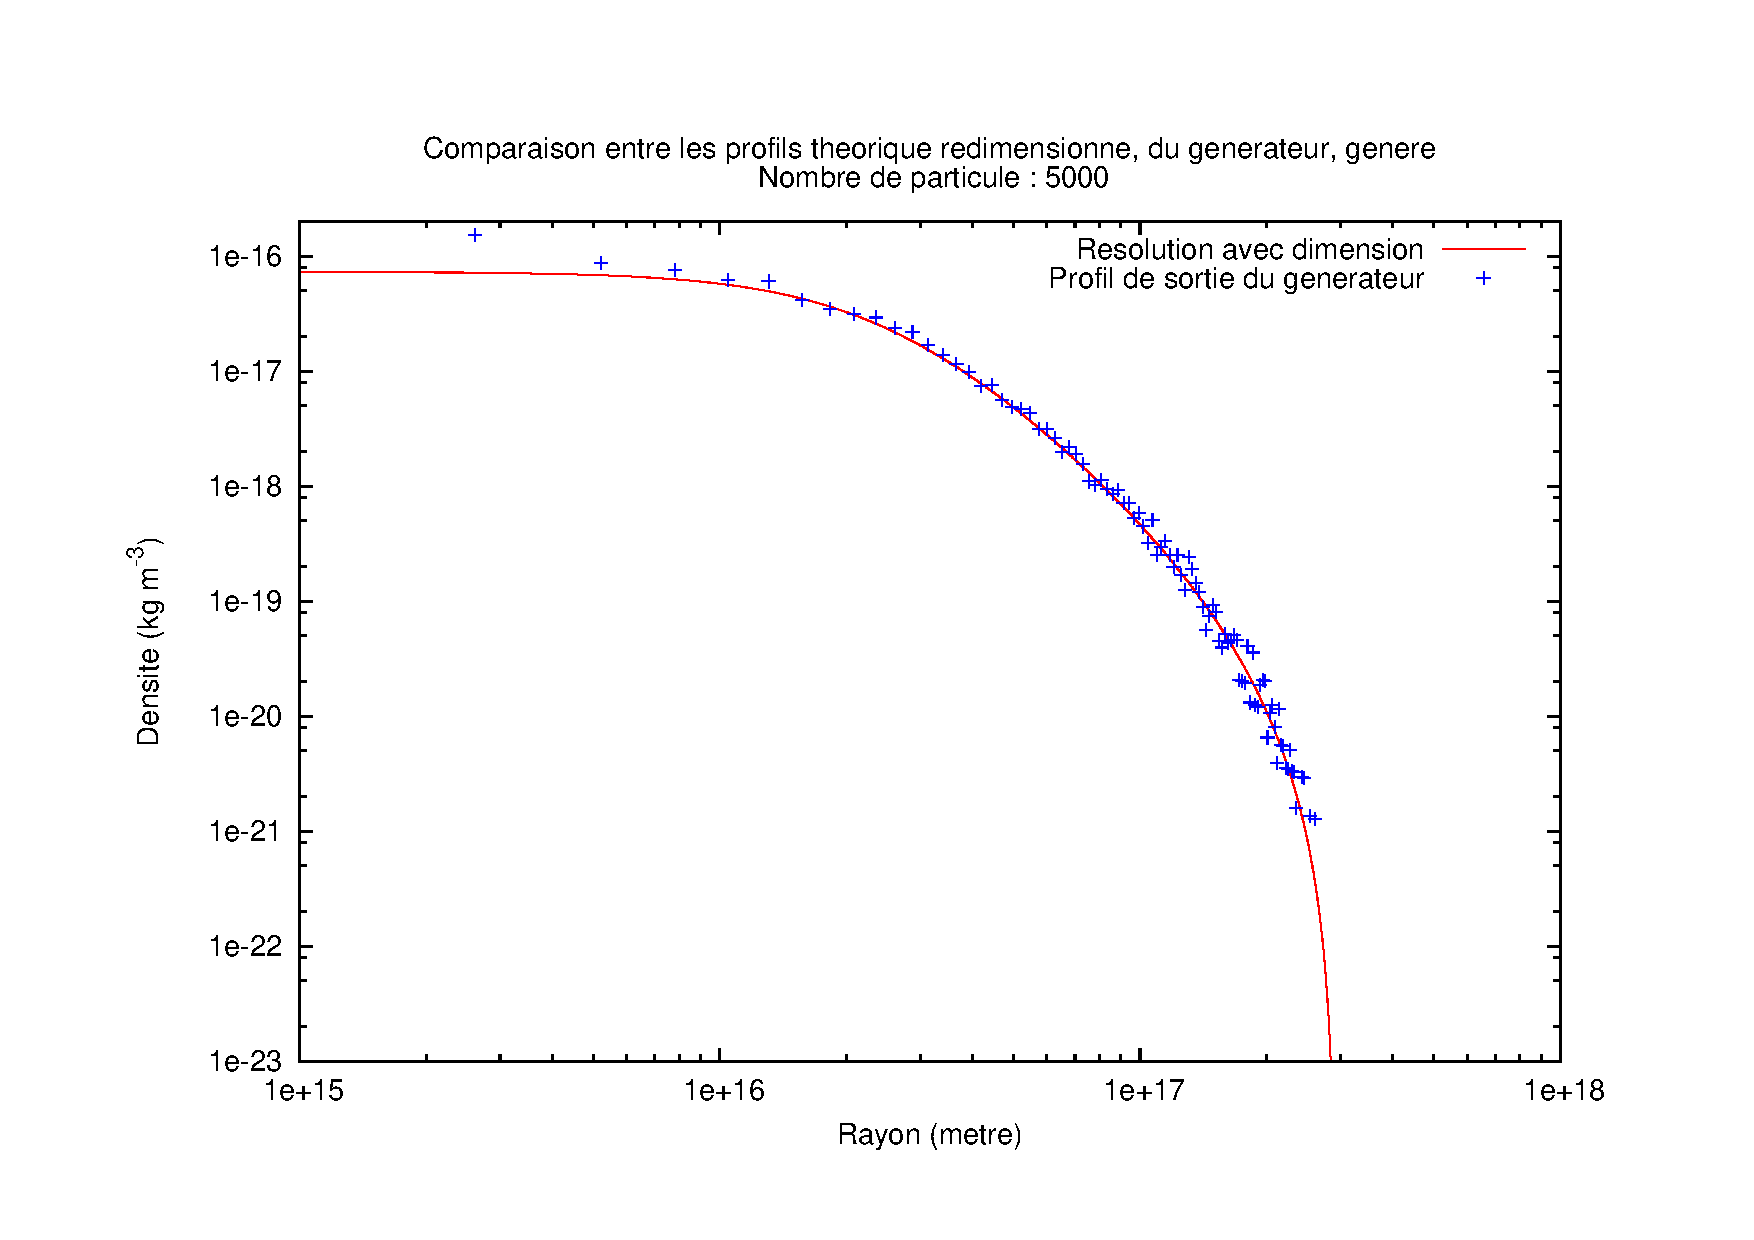
\includegraphics[scale=0.5]{graphe/Comp_dens_gene-theo_5000.pdf}
				% \caption{Comparaison entre la résolution numérique et la densité donnée par le générateur\label{Comp_gene-theo}}
			% \end{figure}
			\begin{figure}[h!]
				% \centering 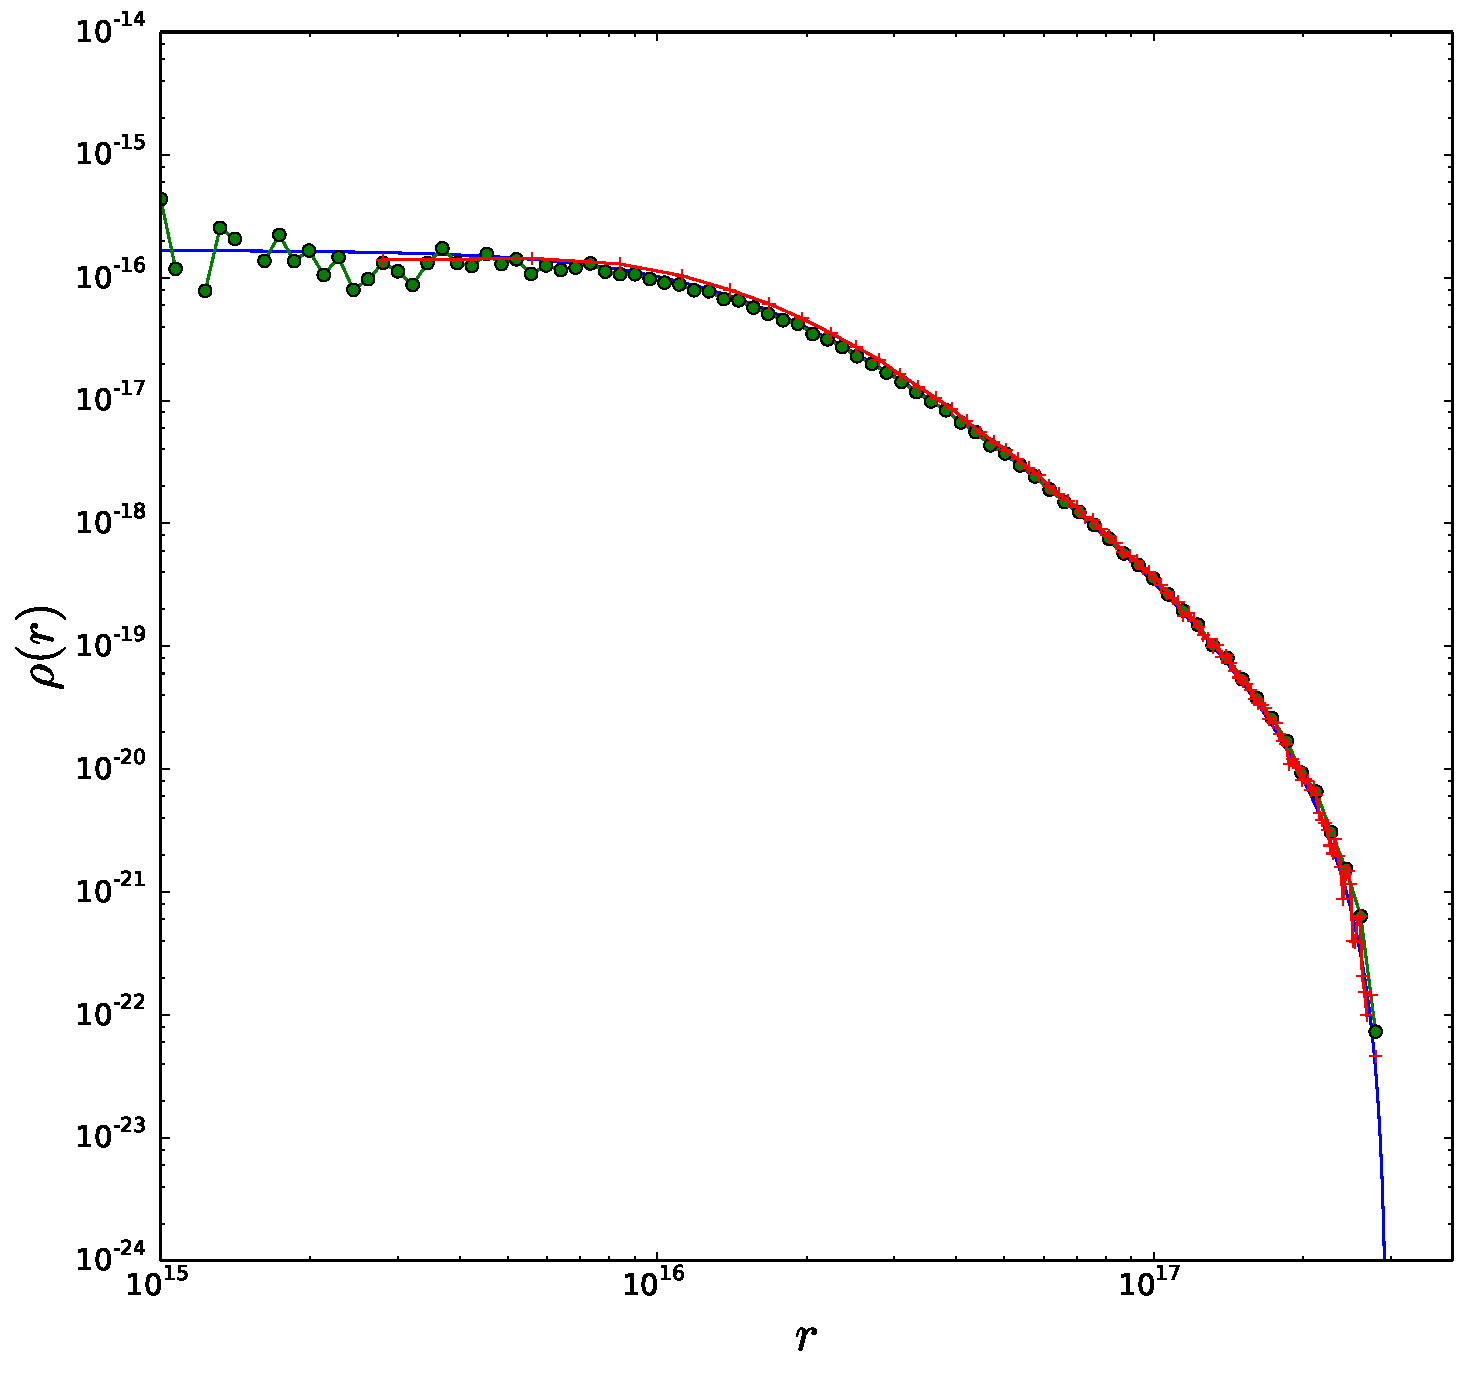
\includegraphics[scale=0.5]{king_model_verification}
				\centering 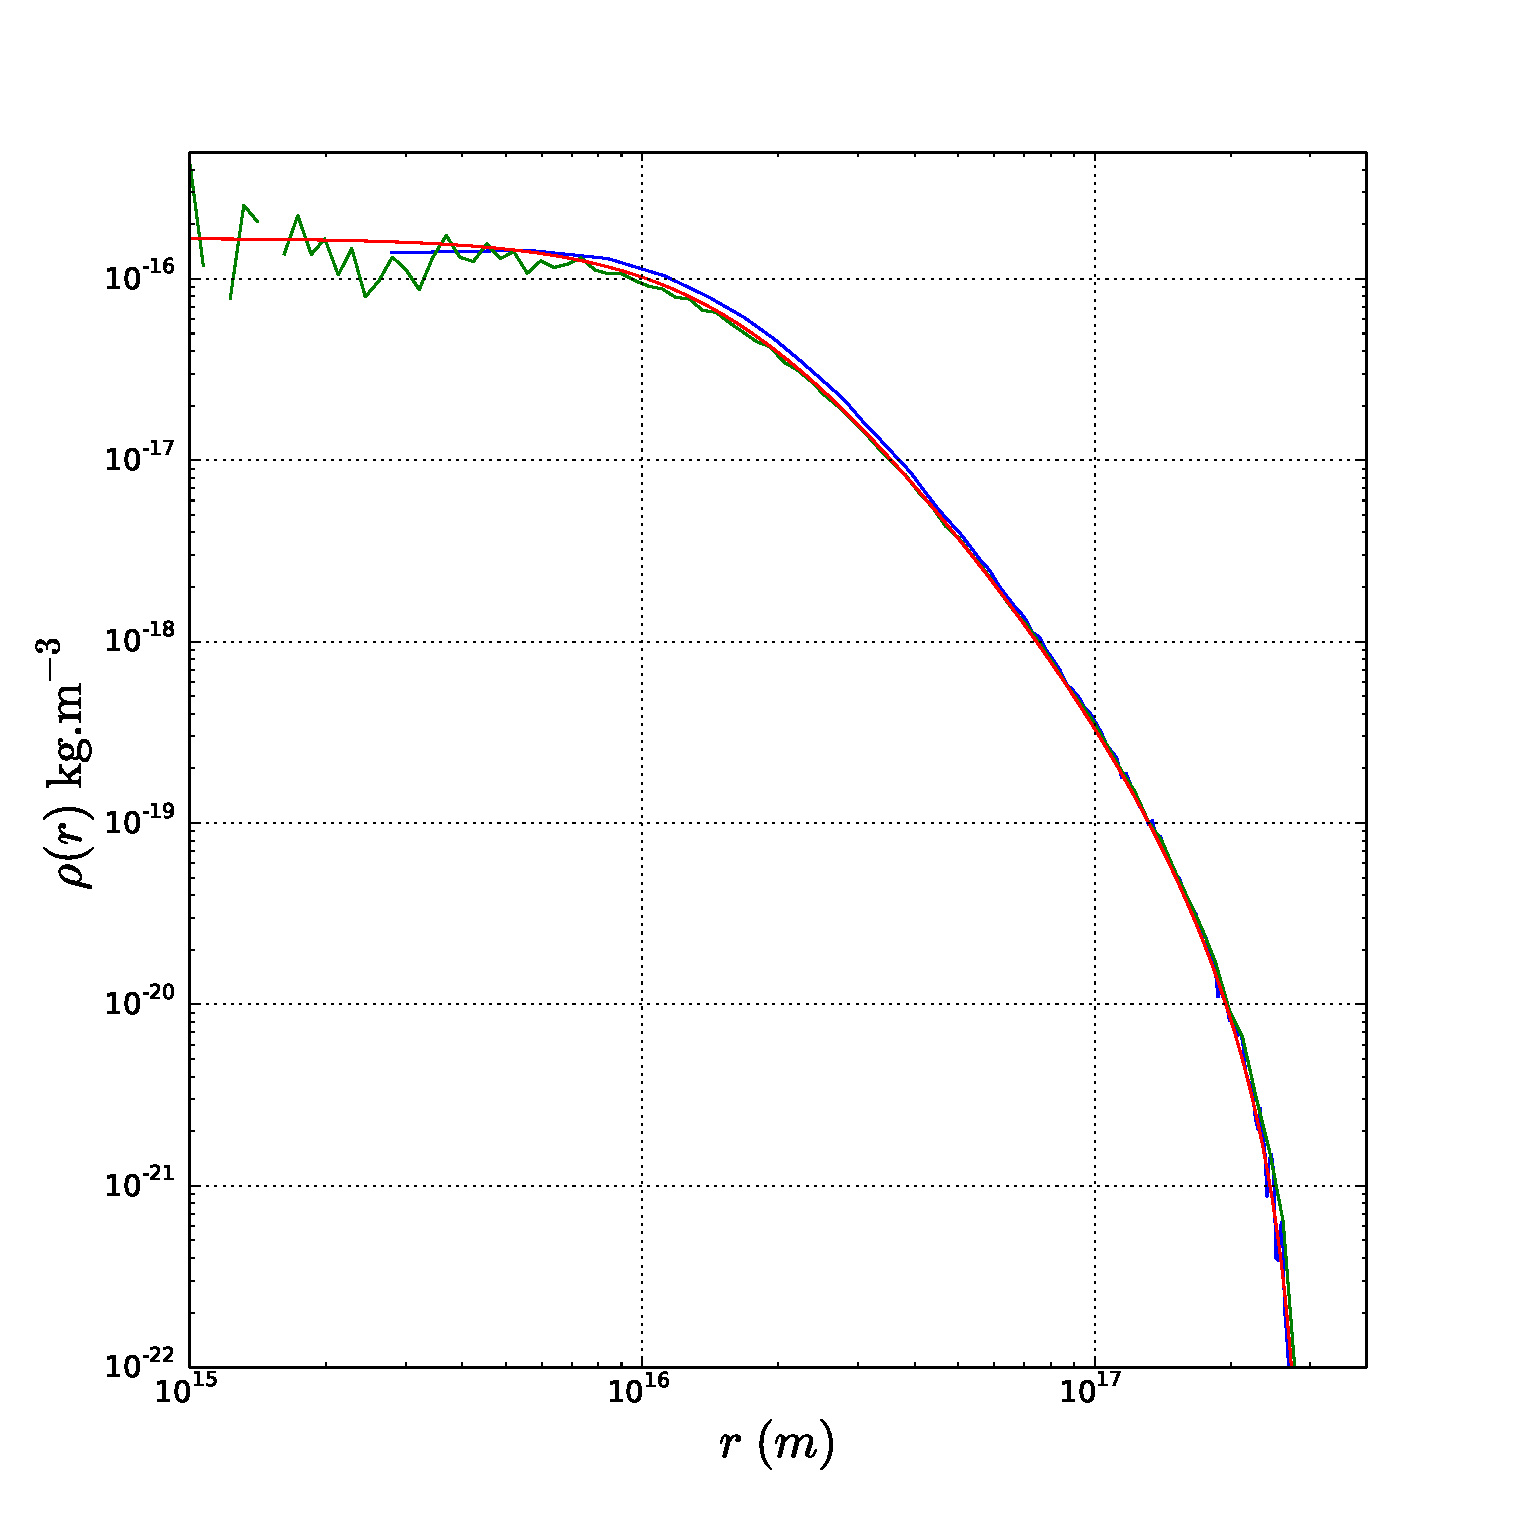
\includegraphics[scale=0.3]{verif_densite.pdf}
				\caption{Comparaison entre la résolution numérique et la densité donnée par le
				générateur\label{Comp_gene-theo}. La courbe rouge correspond à la densité théorique, la
				courbe verte à la densité utilisant les intervalles espacés logarithmiquement et la courbe bleu
				à la méthode décrite ici.}
			\end{figure}

		\subsection{Énergie et potentiel}

			La partie la plus complexe de l'obtention des observables est le calcul de l'énergie. Deux
			choix s'offrent à nous:
			\begin{itemize}
				\item la méthode force brute dans laquelle nous calculons l'énergie totale en utilisant
					l'expression newtonienne du potentiel:
					$$
						E_{tot} = \frac{1}{2}\sum_{i = 1}^{N} m_i v_i^2 - G \sum_{i = 1}^{N} \sum_{j < i}^N \dfrac{m_i m_j}{|| r_i - r_j ||}
					$$
					avec $N$ le nombre de particule. Le problème de cette méthode est qu'elle nécessite $N^2$
					opérations et n'est donc pas opérationnelle lorsque nous travaillons avec un grand
					nombre de particules.
					% De plus, si deux particules sont très proches, l'énergie
					% potentielle va diverger.

				\item la méthode utilisant l'octree décrit précédemment.
		\end{itemize}
		C'est cette dernière méthode que nous avons utilisée. Nous allons parcourir l'arbre comme décrit dans la
		section~\ref{Sec::KdTree}. Lorsque nous arrivons sur une feuille, nous calculons les interactions de chaque
		particules avec celle dont nous voulons le potentiel. Lorsqu'un cube possède un diamètre angulaire trop
		faible, les particules qu'il contient sont ramenées à une macro particules ayant pour position leur centre
		de masse et comme masse la masse totale des particules du cube. La figure~\ref{potentiel_5000} montre le
		potentiel théorique superposé au modèle de King décrit plus haut.

		En plus du potentiel, nous en profitons pour calculer l'énergie cinétique pour obtenir finalement
		l'énergie totale du système et le rapport du Viriel.

		% c'est le centre de masse des particules qu'il  conti

			% \begin{itemize}
				% \item la méthode force brute : nous calculons l'énergie totale en utilisant
					% l'expression newtonienne du potentiel :
					% $$
						% E_{tot} = \frac{1}{2}\sum_{i = 1}^{N} m_i v_i^2 - G \sum_{i = 1}^{N} \sum_{j < i} \dfrac{m_i m_j}{|| r_i - r_j ||}
					% $$
					% avec $N$ le nombre de particule Le problème de cette méthode est qu'elle nécessite $N^2$
				% opérations et n'est donc pas intéressante lorsque nous travaillons avec un grand
				% nombre de particules. De plus, si deux particules sont très proche,
				% l'énergie potentielle va diverger.
				% \item la réflexion : nous avons déjà calculé la densité, et nous avons
					% la fonction de masse, nous avons tout ce qu'il nous faut pour
					% avoir le potentiel à partir de l'équation de \textsc{Poisson}.
			% \end{itemize}

			% Nous allons calculer le potentiel en résolvant l'équation de \textsc{Poisson}. Voyons
			% comment la résoudre avec ce que nous avons.
			% \begin{align}
				% \Delta\psi &= \frac{1}{r^2}\dfrac{d}{dr}\( r^2 \dfrac{d \psi(r)}{dr} \) = 4\pi G \rho(r) \notag \\
				% r^2 \dfrac{d \psi(r)}{dr} &= 4\pi G \int_0^r \rho(r) r^2 dr = G M(r) \notag \\
				% \intertext{La densité est une fonction continue par morceau, nous pouvons donc écrire :}
				% M(r)    &= 4\pi \int_0^r \rho(r) r^2 dr \notag \\
					% &= 4\pi \sum_{j = 0}^{i - 1} \int_{j \mathrm{dr}}^{(j+1)\mathrm{dr}} \rho_j r^2 dr + 4\pi \int_{r_{i-1}}^r r^2 dr \text{, $r\in\left[ r_{i - 1}; r_i \right]$} \notag \\
					% &= 4\pi \sum_{j = 0}^{i - 1} \rho_j \left[ \dfrac{r^3}{3} \right|_{j \mathrm{dr}}^{(j+1)\mathrm{dr}} + 4\pi\rho_i\left[\dfrac{r^3}{3}\right|_{r_{i - 1}}^{r} \notag \\
					% &= 4\pi \sum_{j = 0}^{i - 1} \dfrac{\rho_j}{3} \mathrm{dr}^3 \( (j+1)^3 - j^3)\) + \dfrac{4\pi \rho_i}{3} \(r^3 - i^3\mathrm{dr}^3\) \notag \\
					% &= M(r_{i-1}) + \dfrac{4\pi \rho_i}{3} \(r^3 - i^3\mathrm{dr}^3\) \notag \\
				% \intertext{Ceci nous permet alors d'écrire le potentiel :}
				% \psi(r) - \psi(0) &= G \int_0^r \dfrac{M(r)}{r^2} dr \notag \\
				% \psi\(r_i\) - \psi(0) &= G \sum_{j = 0}^{i} \left\{\int_{j \mathrm{dr}}^{(j+1)\mathrm{dr}} \dfrac{M(r_{j-1})}{r^2} + \dfrac{4\pi \rho_j}{3 r^2} \(r^3 - j^3\mathrm{dr}^3\) dr\right\} \notag \\
				% \intertext{avec $ r_i = (i+1) \mathrm{dr} $}
				% \psi(r_i) - \psi(0) &= G \sum_{j = 0}^{i} \left\{M_{j-1} \left[ \dfrac{-1}{r}\right|_{j \mathrm{dr}}^{(j+1)\mathrm{dr}} + \dfrac{4\pi \rho_j}{3} \( \left[ \dfrac{r^2}{2} \right|_{j \mathrm{dr}}^{(j+1)\mathrm{dr}} - j^3\mathrm{dr}^3 \left[ \dfrac{-1}{r}\right|_{j \mathrm{dr}}^{(j+1)\mathrm{dr}} \)\right\} \notag \\
						    % &=  G \sum_{j = 0}^{i} \left\{\dfrac{1}{j ( j + 1 ) \mathrm{dr}} \( M_{j - 1} - \dfrac{4\pi \rho_j}{3}j^3\mathrm{dr}^3 \) + \dfrac{4\pi \rho_j}{6}\( 2 j + 1 \)\mathrm{dr}^2\right\}
				% \intertext{Pour le bin central $j = 0$, nous avons :}
				% \psi(dr) - \psi(0)  &=  G \dfrac{4\pi \rho_0}{6}\mathrm{dr}^2
			% \end{align}

			% Pour obtenir la constante $\psi(0)$, nous allons nous servir des conditions sur le bord du système. En effet, nous avons vu plus haut que :
			% \begin{align}
				% \psi_\mathrm{max} = \psi(R) &= - \frac{G M}{R} \\
				% \intertext{Donc :}
				% \psi(R) + \psi(0) - \psi(0) &= - \frac{G M}{R} \\
				% \psi(0) &= - \frac{G M}{R} - \(\psi(R) - \psi(0)\) \\
				% \psi(0) &= \frac{E_l}{m} - \(\psi(R) - \psi(0)\)
			% \end{align}

			% Le graphique~\ref{potentiel_5000} nous montre le potentiel théorique et le potentiel calculé par cette méthode.

			\begin{figure}[h!]
				% \centering 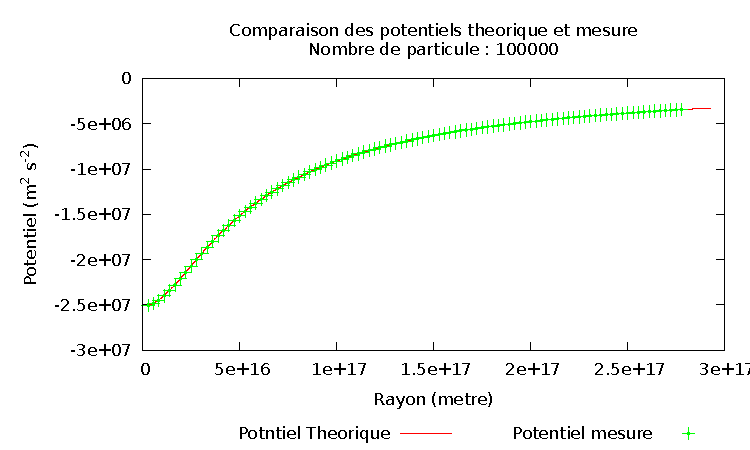
\includegraphics{graphe/Potentiel_ci-100000.pdf}
				\centering 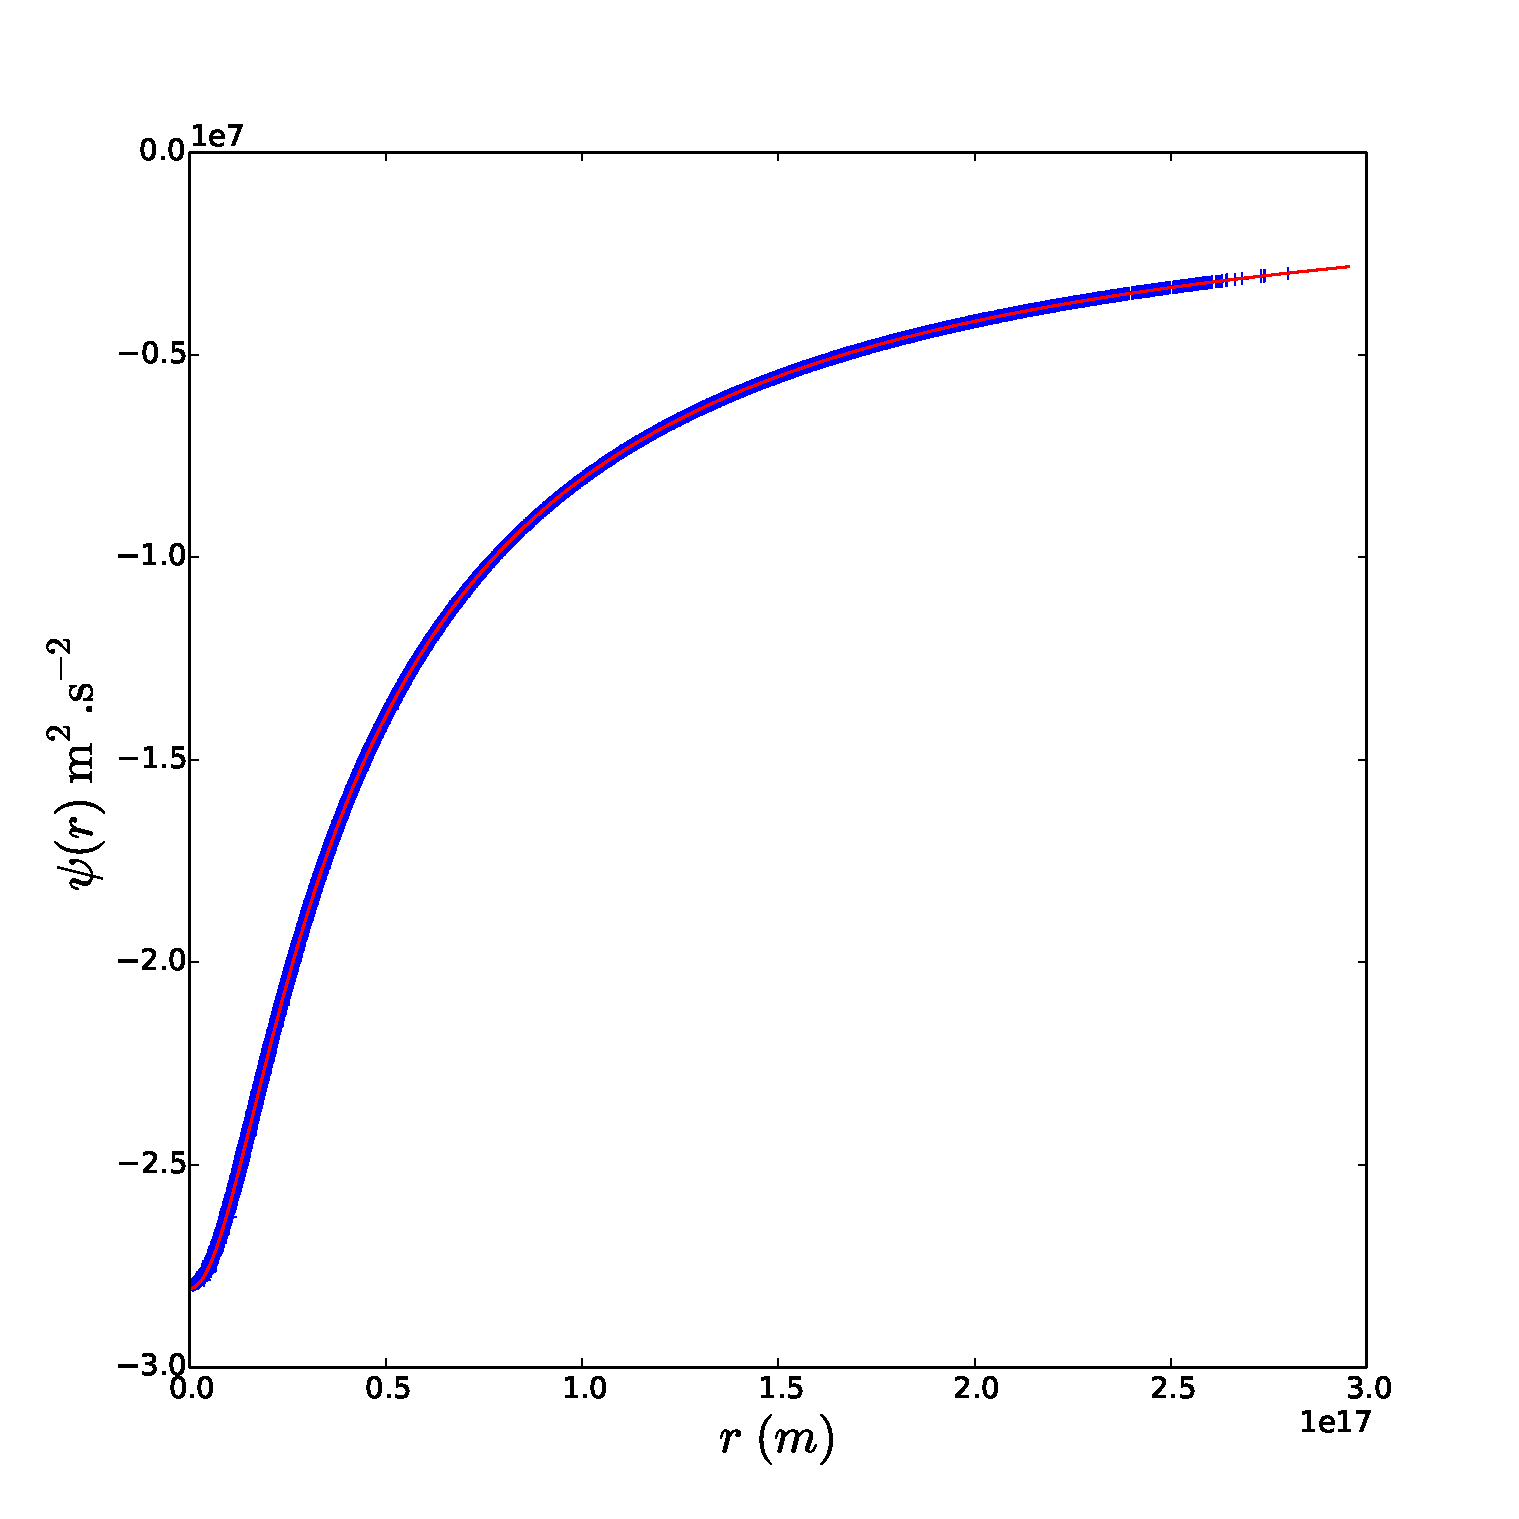
\includegraphics[scale=0.4]{verif_potentiel.pdf}
				\caption{Comparaison entre le potentiel théorique (courbe rouge) et le potentiel donné par le
					générateur (courbe bleu)\label{potentiel_5000}.}
			\end{figure}

		\subsection{Anisotropie des vitesses et forme de l'amas}

			Nos conditions initiales seront généralement des systèmes sphériques et isotrope en vitesse, mais
			qu'en est-il de l'état final?
			Afin de suivre l'évolution de la forme et de l'anisotropie des vitesses de nos système au cours
			du temps, nous avons dévellopé deux observables:
			% Pour savoir si les systèmes sont resté dans ces conditions ou ont
			% vu leurs forme ou distribution de vitesse changer, nous calculons en plus deux autres quantités:
			l'indicateur d'anisotropie et les rapport d'axe de la matrice d'inertie.

			L'indicateur d'anisotropie des vitesses est défini comme suit:
			\begin{align}
				\beta(r) = 1 - \dfrac{\sigma_t^2(r)}{2\sigma_r^2(r)}
			\end{align}
			avec $\sigma_t$ la dispersion de vitesse tangentielle et $\sigma_r$ la dispersion de vitesse
			radiale. Pour obtenir ces dispersions, nous calculons, pour chacune des coquilles de la
			figure~\ref{schema::bin}, les vitesses tangentielles moyennes et les vitesses radiales moyennes,
			puis les dispersions de vitesses correspondantes.
			Lorsque $\beta(r) \equiv 0$, le système est isotrope, pour $\beta(r) \rightarrow 1$ le système
			est radial en vitesse et enfin quand $\beta(r) < 0$ le système est tangentiel.
			Cet indicateur va nous permettre de déceler l'apparition d'une éventuelle instabilité
			d'orbite radiale.

			% Le dernier point à vérifier est la conservation de la sphéricité de nos systèmes. En effet, sauf
			% dans le cas de conditions particulière, comme une instabilité d'orbite radiale, la forme
			% sphérique doit être conservée au cours de l'évolution, voir~\citet{JPerez96}.
			% Maintenant que la densité et le potentiel de l'amas
			% généré ont été vérifiés, il faut aussi vérifier que
			% l'amas ne change pas de forme : nous générons un amas
			% sphérique, nous devons~\footnote{il a en effet été
			% montré qu'un \textsc{King} non collisionnel est
			% stable~\citet{JPerez96}} conserver un amas sphérique
			% après l'avoir fait évoluer.
			% Pour vérifier que la forme
			% de l'amas ne change pas, nous allons regarder comment
			% évoluent les axes principaux d'inertie. Pour ce faire,
			% nous allons calculer les valeurs propres \mbox{$\lambda_1 > \lambda_2 > \lambda_3$} de la matrice
			% d'inertie:
			Pour surveiller l'évolution de la forme du système, nous calculons les valeurs propres
			\mbox{$\lambda_1 > \lambda_2 > \lambda_3$} de la
			matrice d'inertie:
			\begin{align*}
				% \mathfrak{I} &= \(\begin{array}{ccc}
							% \int \(y^2 + z^2\) dm & - \int xy dm & - \int xz dm \\
							% -\int xy dm & \int \(x^2 + z^2\) dm & - \int yz dm \\
							% -\int xz dm & -\int yz dm & \int \(x^2 + y^2\) dm
						% \end{array}\) \\
				% \intertext{avec $dm$ l'élément de masse.}
				\mathfrak{I}   = \(\begin{array}{ccc}
							A & - D & - E \\
							-D & B & - F \\
							-E & -F & C
						\end{array}\)
				% \intertext{L'équation aux valeurs propres va alors s'écrire :}
				% \left|\mathfrak{I} - \lambda \mathbb{I}\right|  &= \(A - \lambda\)\left[\(B-\lambda\)\( C-\lambda\) - F^2\right] + D \(-D\(C-\lambda\) - F E\) - E \left[ D F + E\(B - \lambda\)\right] \notag
				\intertext{avec:}
				\begin{array}{cc}
					\displaystyle A = \sum_{i= 1}^N y_i^2 + z_i^2  &
					\displaystyle D = \sum_{i= 1}^N x_iy_i  \\
					\displaystyle B = \sum_{i= 1}^N x_i^2 + z_i^2  &
					\displaystyle E = \sum_{i= 1}^N x_iz_i  \\
					\displaystyle C = \sum_{i= 1}^N y_i^2 + x_i^2  &
					\displaystyle F = \sum_{i= 1}^N y_iz_i  \\
				\end{array}
			\end{align*}
			% polynôme d'ordre 3 que l'on résout avec la méthode de \textsc{Cardan}.

			Une fois ces valeurs propres obtenues, nous traçons l'évolution des rapports d'axe (couramment nommés \og axial ratio\fg)
			$a_1 = \lambda_1 / \lambda_2$ et $a_2 = \lambda_3 / \lambda_2$. Quand $a_1 = a_2 = 1$, le
			système est sphérique. Si $a_2 < 1$ et $a_1 = 1$, le système présente une forme allongée
			caratéristique de l'instabilité d'orbite radiale; et enfin, pour $a_1 >
			1$ et $a_2 < 1$ le système est triaxial. Cette observable va donc nous être très utile pour
			détecter l'apparition d'instabilité morphologiques comme l'instabilité d'orbite radiale.
			% les
			% valeurs propres étant numérotées dans l'ordre
			% décroissant .

		\subsection{Température}

			La dernière observable que nous souhaitons obtenir est la température. La température que nous
			calculons est la version discréte de celle donnée dans le chapitre~\ref{King::Chapitre}:
			\begin{align}
				T(r) &= \dfrac{\displaystyle\int_{-\infty}^{\infty}v^2 f(\vec{x}, \vec{p})\vdp}{\displaystyle\int_{-\infty}^\infty\vdr\int_{-\infty}^{\infty}f(\vec{x}, \vec{p})\vdp} \\
				     &= \dfrac{\displaystyle\int_{-\infty}^{\infty}4\pi v^4 f(\vec{x}, \vec{p})\dx{v}}{\displaystyle\int_{-\infty}^\infty\vdr\rho(r)} \\
				T(r) &\simeq \dfrac{\displaystyle\sum_i 4\pi v_i^4 f(r, v_i)}{\displaystyle\int_{-\infty}^\infty\vdr\sum_i 4\pi v_i^2 f(r, v_i)} \\
				     &= \dfrac{\displaystyle\sum_i v_i^2 \rho(r)}{\displaystyle\sum_i 4\pi r_i^2 \rho(r_i)dr}
			\end{align}
			Cette observable va nous permettre de savoir si les sphères sont chauffées ou refroidies par leurs
			interactions avec un bain thermique, et à quelle rythme.

	%\section{Résultat des simulations}
		%Les seules simulations que nous avons pu faire dans le cadre du stage sont des tests pour vérifier la stabilité de nos conditions initiales, ce qui représente déjà un travail important.

Nous avons donc commencé par générer des amas comportant un faible nombre de particules (~1000 ou 5000 particules~) afin de vérifier notre générateur, ce sont les résultats montrés par la courbe~\ref{Comp_gene-theo} pour 5000 particules, puis~\ref{potentiel_5000} pour 100000 particules.
Il nous faut maintenant vérifier que ces amas restent stables sur un grand nombre de temps dynamiques. Les simulations présentées dans cette section utilisent un amas réel dont les données ont été récupéré dans le catalogue de
\textsc{Harris} et à partir du travail fait dans les chapitres précédents. Il s'agit de l'amas NGC 288. Pour cet amas, les calculs analytiques donnent $\alpha = 439.72$.

Passons maintenant à l'étude de la stabilité sur le "long" terme de nos amas. Nous montrerons ici les résultats des tests
décrits dans la section~\ref{Verif_gene}.

Dans la table~\ref{eps_Neps}, nous avons indiqué quelles valeurs de $\epsilon$ nous avons utilisées : la valeur de $N_\epsilon$ correspondante, le nombre de particules qui sont au-delà du rayon des conditions initiales de l'objet,
et quelques autres informations utiles pour trouver la valeur qui nous intéresse.
	\begin{table}[h!]
		\begin{center}
			\begin{tabular}{|c|c|c|c|c|c|}
				\hline
				\multirow{2}{1cm}{$\epsilon\ \(pc\)$}	&	\multirow{2}{1cm}{$N_\epsilon$}	&	\multirow{2}{1cm}{$N_\mathrm{out}$}	&	\multirow{2}{3.5cm}{Fraction d'énergie cinétique emportée}	&	\multirow{2}{3.5cm}{Fraction d'énergie potentielle emportée}	&	\multirow{2}{2cm}{Courbes associées} \\
					&	&	&	&	&	\\
				\hline
				\hline
				$0.0194028$	&	$ 0.44 $		&	380	&	$ 0.00013573$			&	$ 0.00081092$	&	\ref{soft::0.019}, \ref{soft::0.019-Ax}\\
				\hline
				$0.05$		&	$ 7.52 $		&	239	&	$ 8.04628\times 10^{-5}$	&	$ 0.000488421$	&	\ref{soft::0.05}, \ref{soft::0.05-Ax}\\
				\hline
				$0.15$		&	$ 203.17 $		&	282	&	$ 9.91201\times 10^{-5}$	&	$ 0.00106241$	&	\ref{soft::0.15}, \ref{soft::0.15-Ax}\\
				\hline
				$0.20$		&	$ 481.58 $		&	653	&	$ 0.000265688$			&	$ 0.00265207$	&	\ref{soft::0.2}, \ref{soft::0.2-Ax}\\
				\hline
				$0.30$		&	$ 1625.34 $		&	919	&	$ 0.000433181$			&	$ 0.00466071$	&	\ref{soft::0.3}, \ref{soft::0.3-Ax}\\
				\hline
			\end{tabular}
		\end{center}
		\caption{Valeurs testés pour $\epsilon$ et $N_\epsilon$\label{eps_Neps}}
	\end{table}

	Discutons maintenant les résultats.

	\begin{description}
	%\paragraph{$\epsilon = 0.0194028$ :}
	\item[$\epsilon = 0.0194028$]
	Ce paramètre donne des résultats satisfaisants : sa densité évolue assez peu sur le temps de la simulation comparé aux valeur de $\epsilon > 0.05$, et ses axes d'inertie restent constant
	(~le bruit visible sur les graphes est dû au bruit statistique, bruit statistique dû au nombre fini de particules~). Par contre, le nombre de particules dans un volume de taille $\epsilon$ est trop petit : nous sommes trop loin de la limite fluide.

	%\paragraph{$\epsilon = 0.05$ :}
	\item[$\epsilon = 0.05$]
	Les fractions d'énergie potentielle et cinétique emportées par les particules sortantes sont minimum pour ce paramètre. De plus, sa densité et ses axes d'inertie évoluent peu, comme pour la valeur précédente.
	Cette fois, nous avons suffisamment de particules dans le volume de taille $\epsilon$.

\begin{figure}[h!]
	\centering 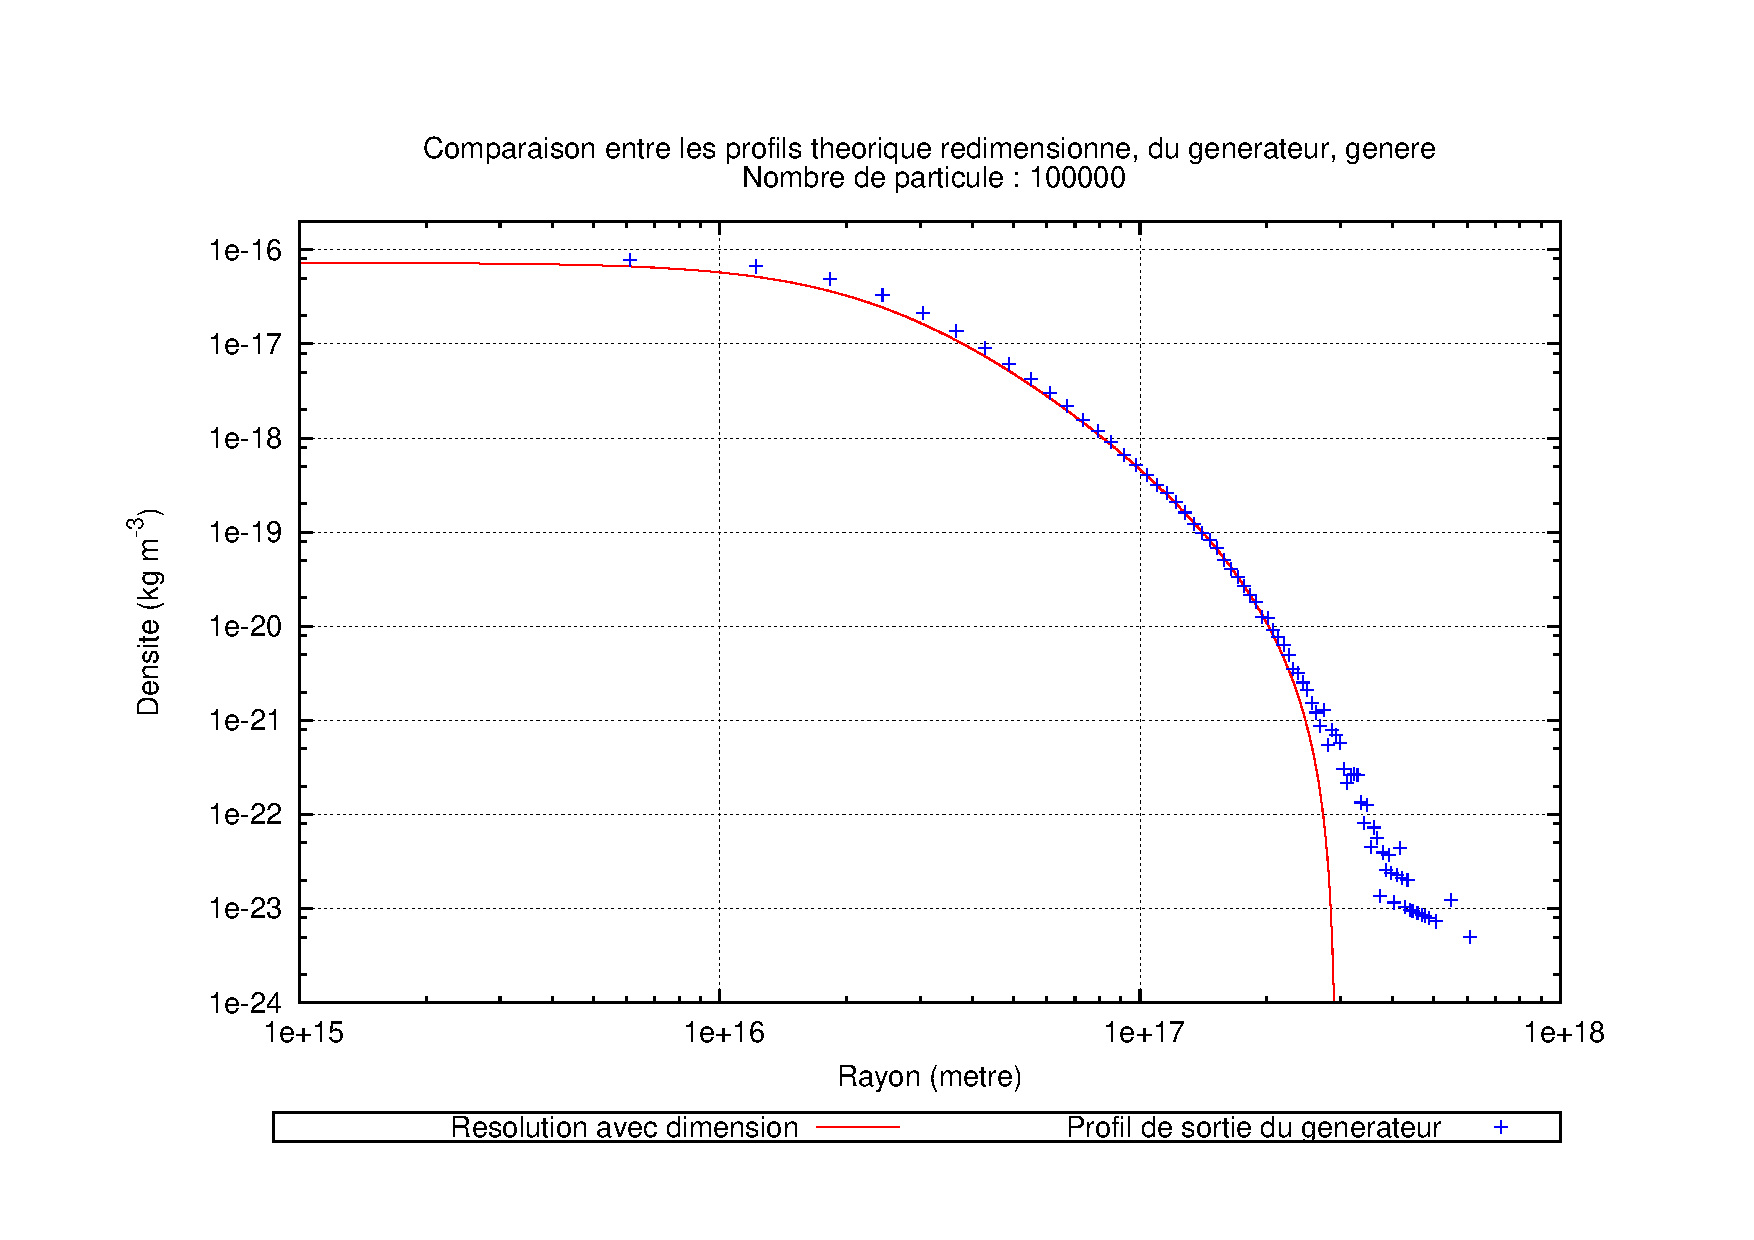
\includegraphics[scale=0.5]{graphe/Comp_dens_gene-theo_0-05.pdf}
	\caption{Comparaison entre la densité numérique et la densité après évolution : $\epsilon = 0.05$\label{soft::0.05}}
\end{figure}

\begin{figure}[h!]
	\centering 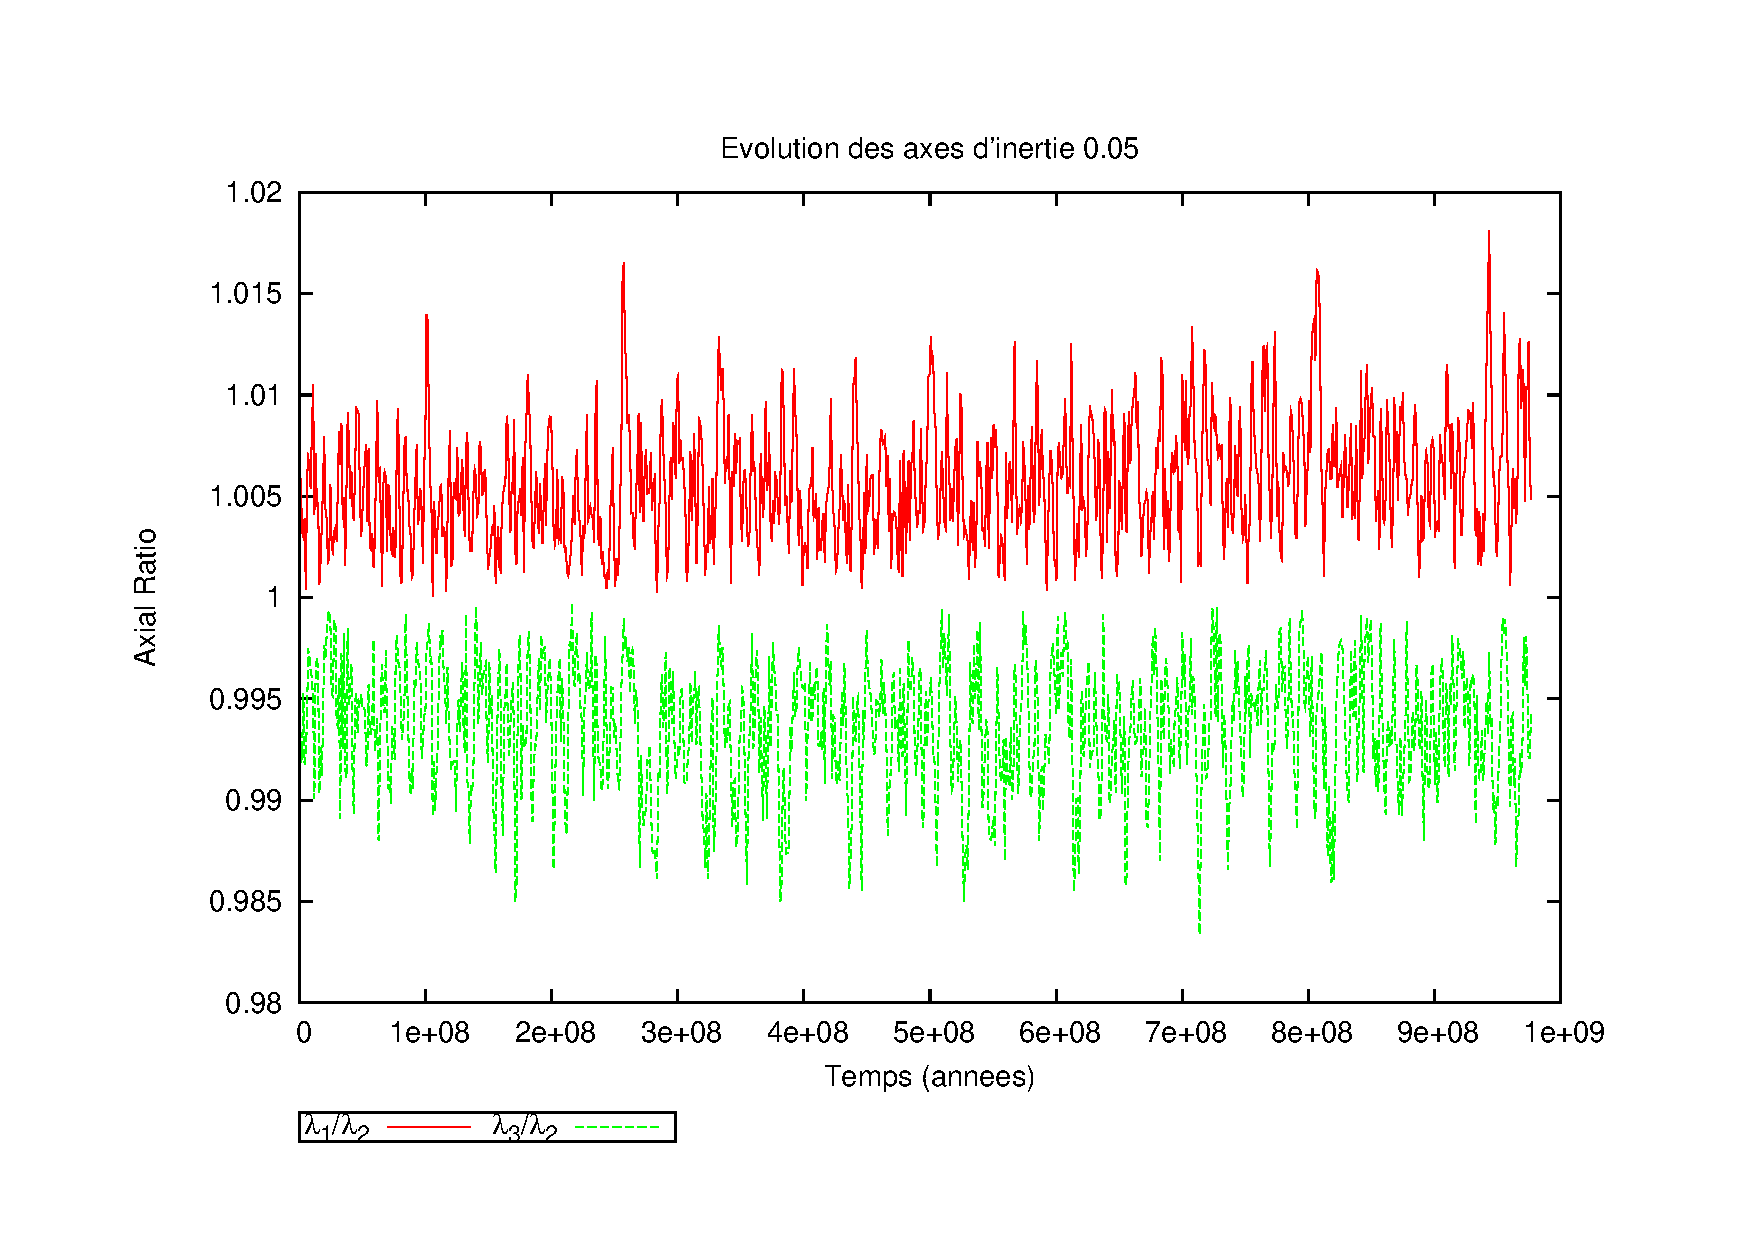
\includegraphics[scale=0.5]{graphe/Axial_ratio_0-05.pdf}
	\caption{Évolution des rapports des axes d'inertie : $\epsilon = 0.05$\label{soft::0.05-Ax}}
\end{figure}

	%\paragraph{$\epsilon = 0.15$ :}
	\item[$\epsilon = 0.15$]
	Pour ce paramètre, la fraction d'énergie potentielle emportée est de l'ordre de $0.1\%$, ce qui représente un changement important pour le rapport du Viriel $2 E_c/E_p$
	(~avec $E_c$ l'énergie cinétique et $E_p$ l'énergie potentielle~) : le profil de densité a complétement changé, l'amas s'est étendu.
	Par contre, il commence à se passer des choses intéressantes au niveau des axes d'inertie : pendant une grande partie de la simulation l'amas conserve sa forme, puis une instabilité arrive et il se déforme. % selon
%	l'un des axes, mais reste constant sur le second.
	\item[$\epsilon > 0.15$]
	Les valeurs supérieurs de $\epsilon$ ne sont alors clairement pas intéressante. De plus, ces valeurs sont trop proches du rayon de cœur de l'amas qui est de l'ordre de $10^{16}\ m = 0.32\ pc$ : en lissant toute
	la partie centrale de l'amas, nous changeons sa dynamique. En effet, il suffit de voir que, en augmentant le paramètre de lissage, l'instabilité menant à une déformation arrive de plus en plus tôt.
	Les déformations deviennent plus violentes.
	\end{description}

	La valeur de lissage optimale se trouve donc entre $\epsilon = 0.05$ et $\epsilon = 0.15$, pour une dizaine de particule (~pour $N_\epsilon = 10$, $\epsilon \sim 0.05497\ pc$~).




\chapter{Comparaison entre Gadget et un code Vlasov\label{Chap::VlasovGadget}}
	\minitoc%

	\todo[inline]{Ce chapitre en est à peine à son premier jet. Toutes les figures ne sont pas encore commenté (ça arrivera dans le courant de la
	semaine). Il manque aussi les figures contenant tous les $j$ sommé.}

	% Une des questions qui se posent avec notre approche concerne sa validité. En effet, à quel point gadget peut il
	% être proche d'un programme résolvant directement les équations de Vlasov-Poisson. Dans ce chapitre, nous tentons
	% d'apporter des éléments de réponse.

	Avant de présenter les résultats obtenus au cours de la thèse, nous allons présenter un travail que nous avons effectué en parallèle. Il a été
	effectué conjointement avec Stéphane Colombi, Thierry Sousbie et Sébastien Peirani. Il consiste à comparer les résultats donnés par un code
	résolvant numériquement l'équation de Vlasov (écrit par Thierry Sousbie en se basant sur~\cite{1983PASJ...35..547F}) et le code $N$-corps
	\textsc{gadget-2}.

	Tous les diagrammes de l'espace des phases, sauf si précisé, présente à gauche la simulation Vlasov et à droite la simulation
	\textsc{gadget-2}. Tous sont normalisés de façon à utiliser la même échelle de couleurs pour une même simulation.

	\section{Description du code Vlasov}

		Nous considérons un système à symétrie sphérique. L'équation de Vlasov s'écrit:
		\begin{align}
			\pderivn{f}{t} + v_r\pderivn{f}{r} + \(\dfrac{j^2}{r^3} - \dfrac{GM(r)}{r^2}\)\pderivn{f}{v_r} = 0\label{Eq::ValGad::Pois}
		\end{align}
		avec $f = f(r, u, j, t)$ la fonction de distribution dans l'espace des phases du système au temps $t$, $r$ le rayon de l'objet, $v_r$
		la vitesse radiale et $j$ le moment angulaire. La fonction $M(r)$ donne la masse contenue à l'intérieur de la sphère de rayon $r$.

		Pour résoudre l'équation, l'espace des phases $\(r, v_r, j\)$ est discrétisé sur un maillage tridimensionnel de dimension $(r, v_r,
		j)\in\(\left[r_\mathrm{min}; r_\mathrm{max}\right], \left[-v_r^\mathrm{max}; v_r^\mathrm{max}\right], \left[0;
		j_\mathrm{max}\right]\)$ avec $r$ évoluant logarithmiquement. Chaque point du maillage est considéré comme une particule.
		L'équation~\refeq{Eq::ValGad::Pois} est séparée en deux opérateurs:
		\begin{itemize}
			\item un premier opérateur permet d'obtenir la trajectoire d'une particule libre:
				\begin{align*}
					\pderivn{f}{t} + v_r\pderivn{f}{r} + \dfrac{j^2}{r^3}\pderivn{f}{u} = 0
				\end{align*}
			\item un second permettant de calculer l'accélération:
				\begin{align*}
					\pderivn{f}{t} - \dfrac{GM(r)}{r^2}\pderivn{f}{v_r} = 0
				\end{align*}
		\end{itemize}
		Ces deux opérateurs, alliés à un schéma de type \og\sm\fg, % \og{}Leap-frog\fg,
		vont permettre de faire évoluer la position chaque
		point du maillage du temps $t$ au temps $t+dt$. Puis, profitant du fait que toutes les couche de moment angulaire est indépendante des
		autres, une interpolation de la fonction de distribution dans le plan $\(r, v_r\)$ pour chaque $j$ permet de reconstruire le maillage.

		L'axe selon $r$ évoluant logarithmiquement, un problème va se poser lorsque $r\to0$. Pour l'éviter, nous faisons l'approximation que
		les particules à l'intérieur du rayon $r_\mathrm{min}$ sont libres. Ce rayon doit donc être suffisamment petit pour que cette approximation
		soit vérifié, mais suffisamment grand pour éviter la divergence du logarithme.
		% toutes les particules passant sous ce rayon $r_\mathrm{min}$ puissent évoluer comme des particules libres.

		Plus de détails sur le fonctionnement du code pourront être trouvés dans l'article associé à cette étude (référence?). Pour effectuer
		la comparaison de ce code à \textsc{gadget-2}, nous allons utiliser une sphère de Hénon de viriel $\gamma$. À cause de certaines limitations
		inhérentes à l'interpolation, nous avons dû lisser cette sphère en multipliant la fonction de distribution par la fonction:
		\begin{align*}
			g(r) = \mathrm{erf}\( \dfrac{R - r }{ r_\epsilon }\) + 1
		\end{align*}
		avec $R$ est le rayon de l'objet et $r_\epsilon$ le rayon sur lequel la sphère sera lissée.

		Dans les sections suivantes, nous allons comparer ces deux codes en utilisant deux rapports du viriel: $\gamma=-0,5$ et $\gamma=-0,1$.
		% l'évolution de la sphère de Hénon avec un viriel de $\gamma=-0,5$ puis nous
		% enchaînerons sur une comparaison utilisant un viriel de $\gamma=-0.1$.

	\section{Comparaison pour $\gamma = -0,5$}

		Nous allons commencer par comparer nos deux codes numériques dans le cadre de conditions initiales dont l'évolution est bien connue et
		décrite dans la littérature: nous allons regarder/étudier l'effondrement d'une sphère de Hénon de viriel $\gamma=-0,5$. Nous prenons comme
		référence l'article de~\cite{1983PASJ...35..547F}. Nous nous placerons dans le même système d'unités.

		Pour comparer nos simulations, nous nous baserons sur la correspondance entre l'espace des phases $(r, v_r)$ pour $j=0,425$, l'espace
		des phases intégré sur $j$ et l'évolution du profil de densité de l'objet. Nous effectuerons ces comparaison à différents temps afin
		de montrer que nous obtenons bien le même comportement au cours du temps. La simulation \textsc{gadget-2} utilisée ici comporte $10^6$
		particules. L'article associé étudiera aussi l'évolution de simulations composées de $10^5$ et $10^7$ particules.

		\todo[inline]{L'impact du lissage de la force. À rédiger selon ce qui est dit dans l'article. Pas possible de présenter l'étude sur le
		pas de temps, je n'ai rien d'utilisable.}

		\subsection{Effet du lissage de la force}

			Un paramètre important de la simulation va être le paramètre de lissage de la force $\epsilon$. Ce paramètre va influencer sur
			la dynamique en donnant ou retirant de l'importance au collision. Nous avons donc effectué des simulations d'une sphère de
			Hénon lissée, de viriel $\gamma=-0,5$, avec différents $\epsilon$. La figure~\ref{Fig::ValGad::0.5::SoftAll} montre l'espace
			des phases pour chaque $\epsilon$ utilisé.
			\begin{figure}[htbp]
				\begin{subfigure}{0.5\linewidth}
					\centering 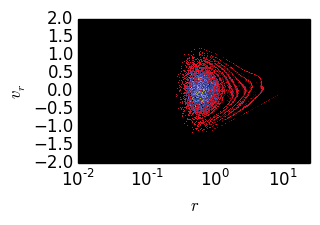
\includegraphics{{vlasov_gadget/Vlasov_0.5_Soft/CompVlasGad_512_0.5_0.0001}.png}
					\centering \caption{$\epsilon=10^{-4}$\label{Fig::ValGad::0.5::Soft1}}
				\end{subfigure}\hfill
				\begin{subfigure}{0.5\linewidth}
					\centering 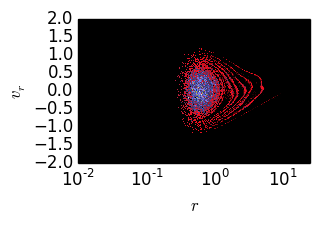
\includegraphics{{vlasov_gadget/Vlasov_0.5_Soft/CompVlasGad_512_0.5_0.001}.png}
					\centering \caption{$\epsilon=10^{-3}$\label{Fig::ValGad::0.5::Soft2}}
				\end{subfigure}
				\begin{subfigure}{0.5\linewidth}
					\centering 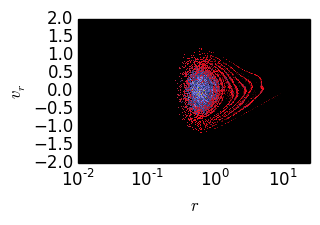
\includegraphics{{vlasov_gadget/Vlasov_0.5_Soft/CompVlasGad_512_0.5_0.01}.png}
					\centering \caption{$\epsilon=10^{-2}$\label{Fig::ValGad::0.5::Soft3}}
				\end{subfigure}\hfill
				\begin{subfigure}{0.5\linewidth}
					\centering 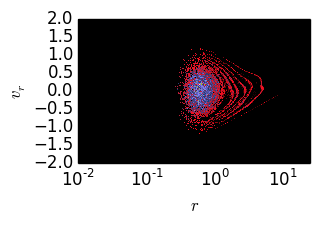
\includegraphics{{vlasov_gadget/Vlasov_0.5_Soft/CompVlasGad_512_0.5_0.1}.png}
					\centering \caption{$\epsilon=10^{-1}$\label{Fig::ValGad::0.5::Soft4}}
				\end{subfigure}
				\caption{Représentation de l'espace des phase à $j=0.425$ et $t=45$ pour $\gamma=-0,5$ et différents
					$\epsilon$.\label{Fig::ValGad::0.5::SoftAll}}
			\end{figure}
			Nous pouvons voir sur ces figures que l'espace des phases est très similaires, et ne semble pas dépendre de la valeur de
			$\epsilon$. Les enroulements à grand $r$ montrent les mêmes variations entre chaque diagrammes.

		\subsection{Comparaison entre les simulations Vlasov et \textsc{Gadget-2}}

			Après avoir montré que le lissage de la force n'avait pas d'influence sur l'évolution du Hénon, nous allons comparer nos
			simulations \textsc{gadget-2} avec les simulations Vlasov en utilisant $\epsilon=10^{-3}$. La première chose que nous
			vérifions est la conservation de la sphéricité de la sphère.
			\begin{figure}[htbp]
				\begin{minipage}{0.45\linewidth}
					\begin{center}
					\centering 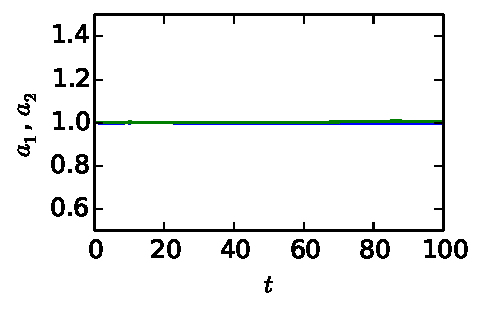
\includegraphics{{vlasov_gadget/AxialRatio_0.5}.pdf}
					\centering \caption{Évolution des rapports d'axes $a_1$ et $a_2$ pour $\gamma=-0,5$.\label{Fig::VlaGad::SpheTest::AR}}
					\end{center}
				\end{minipage}
				\begin{minipage}{0.45\linewidth}
					\begin{center}
					\centering 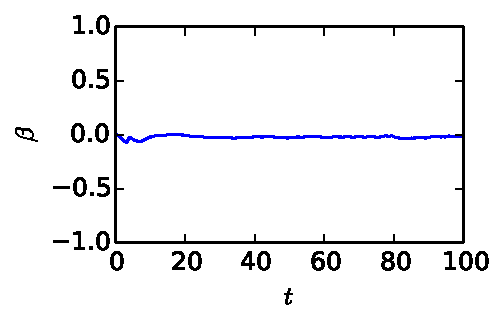
\includegraphics{{vlasov_gadget/Anisotropy_0.5}.pdf}
					\centering \caption{Évolution de l'anisotropie pour $\gamma=-0,5$.\label{Fig::VlaGad::SpheTest::Aniso}}
					\end{center}
				\end{minipage}
			\end{figure}
			C'est ce que montre la figure~\ref{Fig::VlaGad::SpheTest::AR}
			représentant l'évolution des rapports d'axes au cours du temps. Ils restent tous deux très proches de $1$. La sphère de Hénon
			reste bien sphérique tout du long de son évolution. La figure~\ref{Fig::VlaGad::SpheTest::Aniso} montre l'évolution de
			l'anisotropie au cours. Son évolution confire que la sphère conserve son anisotropie tout au long de son évolution.

			Le premier temps que nous regardons est $t=0$. La figure~\ref{Fig::ValGad::0.5::t0} montre l'espace des phases pour les conditions
			initiales. La première chose à noter concerne la différence apparente concernant le maximum de la fonction de distributions. Cette
			différence est dû au faible nombre de particules présentes dans la couche de $j$ choisi. Excepté ce point, nous retrouvons bien la
			croissance progressive du nombre de particule ainsi qu'un étalement progressif des vitesses radiales quand $r$ augmente.
			\begin{figure}[htbp]
				\begin{minipage}{1.00\linewidth}
					\centering \includegraphics[width=\linewidth]{{CompVlasGad_t_0_512_0.5}.png}
					\caption{Comparaison de l'espace des phases entre le code vlasov (à gauche) et le code Gadget (à droite), à $t=0$ et pour $j=0,425$.\label{Fig::ValGad::0.5::t0}}
				\end{minipage}\hfill
				\begin{minipage}{1.00\linewidth}
					\centering \includegraphics{{CompVlasGad_Density_0.5_t_0_error}.pdf}
					\caption{Comparaison du profil de densité entre le code vlasov (en bleu) et le code gadget (en vert), pour $t=0$.\label{Fig::ValGad::0.5::Density::t0}}
				\end{minipage}
			\end{figure}
			\begin{figure}[htbp]
				\centering \includegraphics[width=\linewidth]{{CompVlasGad_t_0_512_0.5_Jall-v2}.png}
				\caption{Espace des phases intégré sur $j$ à $t=0$ pour $\gamma=-0,5$. La simulation vlasov se trouve à gauche, à droite la simulation gadget.\label{Fig::VlaGad::0.5::JAll::t0}}
			\end{figure}
			Du côté du profil de densité (figure~\ref{Fig::ValGad::0.5::Density::t0}), l'accord est très bon, excepté au centre du système où le manque de particules empêche le calcul précis
			de la densité.

			Le deuxième temps que nous avons choisi de montrer se situe peu après la fin de l'effondrement de la sphère de Hénon. Le nombre
			d'enroulement présent sur les graphiques de la figure~\ref{Fig::ValGad::0.5::t13} sont les mêmes. Par contre, l'enroulement central
			donne de la simulation gadget semble un peu en avance sur la simulation vlasov. Ce qui semble confirmé par le \og{}bras\fg s'étendant
			jusqu'à $r=3$ pour la simulation vlasov et jusqu'à $r=4$ pour la simulation gadget.
			\begin{figure}[htbp]
				\begin{minipage}{1.00\linewidth}
					\centering \includegraphics[width=\linewidth]{{CompVlasGad_t_13_512_0.5}.png}
					\caption{Comparaison de l'espace des phases entre le code vlasov (à gauche) et le code Gadget (à droite), à $t=13$ et pour $j=0,425$.\label{Fig::ValGad::0.5::t13}}
				\end{minipage}\hfill
				\begin{minipage}{1.00\linewidth}
					\centering \includegraphics{{CompVlasGad_Density_0.5_t_13_error}.pdf}
					\caption{Comparaison du profil de densité entre le code vlasov (en bleu) et le code gadget (en vert), pour $t=13$.\label{Fig::ValGad::0.5::Density::t13}}
				\end{minipage}
			\end{figure}
			\begin{figure}[htbp]
				\centering \includegraphics[width=\linewidth]{{CompVlasGad_t_13_512_0.5_Jall-v2}.png}
				\caption{Espace des phases intégré sur $j$ à $t=13$ pour $\gamma=-0,5$. La simulation vlasov se trouve à gauche, à droite la simulation gadget.\label{Fig::VlaGad::0.5::JAll::t13}}
			\end{figure}
			Les profils de densité présenté sur la figure~\ref{Fig::ValGad::0.5::Density::t13} montre par contre un très bon accord, excepté au
			bord du système, où le nombre de particules recommence alors à faiblir. L'extension du système en $r$ est aussi visible.
			% \begin{figure}[htpb]
			% \end{figure}
			Cette extension du profil peut-être expliqué par l'éjection d'une fraction des particules hors du système suite aux collisions se
			produisant dans le système.

			Pour terminer la comparaison à ce viriel, nous regardons ce qu'il se passe à $t=45$. À ce moment, le système a eu le temps de se
			stabiliser. Nous remarquons, en regardant la figure~\ref{Fig::ValGad::0.5::t45}, que la simulation gadget présente des
			\og{}vaguelettes\fg sur les enroulements extérieurs qui semble en avance sur la simulation vlasov.
			\begin{figure}[htbp]
				\begin{minipage}{1.00\linewidth}
					\centering \includegraphics[width=\linewidth]{{CompVlasGad_t_45_512_0.5}.png}
					\caption{Comparaison de l'espace des phases entre le code vlasov (à gauche) et le code Gadget (à droite), à $t=45$ et pour $j=0,425$.\label{Fig::ValGad::0.5::t45}}
				\end{minipage}\hfill
				\begin{minipage}{1.00\linewidth}
					\centering \includegraphics{{CompVlasGad_Density_0.5_t_45_error}.pdf}
					\caption{Comparaison du profil de densité entre le code vlasov (en bleu) et le code gadget (en vert), pour $t=45$.\label{Fig::ValGad::0.5::Density::t45}}
				\end{minipage}
			\end{figure}
			\begin{figure}[htbp]
				\centering \includegraphics[width=\linewidth]{{CompVlasGad_t_45_512_0.5_Jall-v2}.png}
				\caption{Espace des phases intégré sur $j$ à $t=45$ pour $\gamma=-0,5$. La simulation vlasov se trouve à gauche, à droite la simulation gadget.\label{Fig::VlaGad::0.5::JAll::t45}}
			\end{figure}


	\section{Comparaison pour $\gamma = -0,1$}

		Comme pour la comparaison précédente, nous allons commencer par vérifier que le système conserve ses propriété de sphéricité et
		d'isotropie.
		\begin{figure}[htbp]
			\begin{minipage}{0.45\linewidth}
				\begin{center}
				\centering 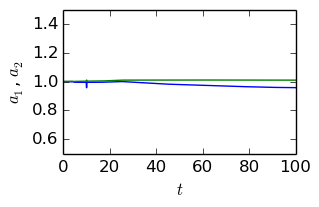
\includegraphics{{vlasov_gadget/AxialRatio_0.1}.pdf}
				\centering \caption{Évolution des rapports d'axes $a_1$ et $a_2$ pour
				$\gamma=-0,1$.\label{Fig::VlaGad::SpheTest::AR0.1}}
				\end{center}
			\end{minipage}
			\begin{minipage}{0.45\linewidth}
				\begin{center}
				\centering 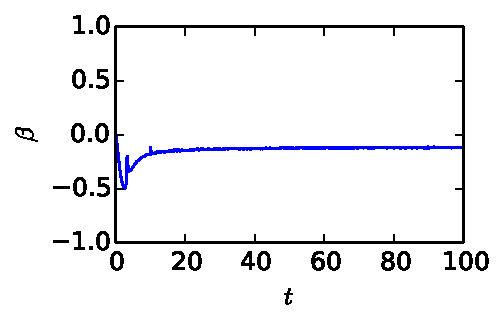
\includegraphics{{vlasov_gadget/Anisotropy_0.1}.pdf}
				\centering \caption{Évolution de l'anisotropie pour $\gamma=-0,1$.\label{Fig::VlaGad::SpheTest::Aniso0.1}}
				\end{center}
			\end{minipage}
		\end{figure}
		C'est ce que montre les figure~\ref{Fig::VlaGad::SpheTest::AR} et~\ref{Fig::VlaGad::SpheTest::Aniso}. Ces deux observables confirment
		donc que l'objet reste bien sphérique et isotrope.

		Le premier temps que nous regardons est $t=0$. La figure~\ref{Fig::ValGad::0.1::t0} montre l'espace des phases pour les conditions
		initiales. La première chose à noter concerne la différence apparente concernant le maximum de la fonction de distributions. Cette
		différence est dû au faible nombre de particules présentes dans la couche de $j$ choisi. Excepté ce point, nous retrouvons bien la
		croissance progressive du nombre de particule ainsi qu'un étalement progressif des vitesses radiales quand $r$ augmente.
		\begin{figure}[htbp]
			\begin{minipage}{1.00\linewidth}
				\centering \includegraphics[width=\linewidth]{{CompVlasGad_t_0_512_0.1}.png}
				\caption{Comparaison de l'espace des phases entre le code vlasov (à gauche) et le code Gadget (à droite), à $t=0$ et pour $j=0,425$.\label{Fig::ValGad::0.1::t0}}
			\end{minipage}\hfill
			\begin{minipage}{1.00\linewidth}
				\centering \includegraphics{{CompVlasGad_Density_0.1_t_0_error}.pdf}
				\caption{Comparaison du profil de densité entre le code vlasov (en bleu) et le code gadget (en vert), pour $t=0$.\label{Fig::ValGad::0.1::Density::t0}}
			\end{minipage}
		\end{figure}
		\begin{figure}[htbp]
			\centering \includegraphics[width=\linewidth]{{CompVlasGad_t_0_512_0.1_Jall-v2}.png}
			\caption{Espace des phases intégré sur $j$ à $t=0$ pour $\gamma=-0,1$. La simulation vlasov se trouve à gauche, à droite la simulation gadget.\label{Fig::VlaGad::0.1::JAll::t0}}
		\end{figure}
		Du côté du profil de densité (figure~\ref{Fig::ValGad::0.1::Density::t0}), l'accord est très bon, excepté au centre du système où le manque de particules empêche le calcul précis
		de la densité.

		Le deuxième temps que nous avons choisi de montrer se situe peu après la fin de l'effondrement de la sphère de Hénon. Le nombre
		d'enroulement présent sur les graphiques de la figure~\ref{Fig::ValGad::0.1::t13} sont les mêmes. Par contre, l'enroulement central
		donne de la simulation gadget semble un peu en avance sur la simulation vlasov. Ce qui semble confirmé par le \og{}bras\fg s'étendant
		jusqu'à $r=3$ pour la simulation vlasov et jusqu'à $r=4$ pour la simulation gadget.
		\begin{figure}[htbp]
			\begin{minipage}{1.00\linewidth}
				\centering \includegraphics[width=\linewidth]{{CompVlasGad_t_5_512_0.1}.png}
				\caption{Comparaison de l'espace des phases entre le code vlasov (à gauche) et le code Gadget (à droite), à $t=5$ et pour $j=0,425$.\label{Fig::ValGad::0.1::t13}}
			\end{minipage}\hfill
			\begin{minipage}{1.00\linewidth}
				\centering \includegraphics{{CompVlasGad_Density_0.1_t_5_error}.pdf}
				\caption{Comparaison du profil de densité entre le code vlasov (en bleu) et le code gadget (en vert), pour $t=5$.\label{Fig::ValGad::0.1::Density::t13}}
			\end{minipage}
		\end{figure}
		\begin{figure}[htbp]
			\centering \includegraphics[width=\linewidth]{{CompVlasGad_t_5_512_0.1_Jall-v2}.png}
			\caption{Espace des phases intégré sur $j$ à $t=5$ pour $\gamma=-0,1$. La simulation vlasov se trouve à gauche, à droite la simulation gadget.\label{Fig::VlaGad::0.1::JAll::t5}}
		\end{figure}
		Les profils de densité présenté sur la figure~\ref{Fig::ValGad::0.1::Density::t13} montre par contre un très bon accord, excepté au
		bord du système, où le nombre de particules recommence alors à faiblir. L'extension du système en $r$ est aussi visible.
		% \begin{figure}[htpb]
		% \end{figure}
		Cette extension du profil peut-être expliqué par l'éjection d'une fraction des particules hors du système suite aux collisions se
		produisant dans le système.

		Pour terminer la comparaison à ce viriel, nous regardons ce qu'il se passe à $t=45$. À ce moment, le système a eu le temps de se
		stabiliser. Nous remarquons, en regardant la figure~\ref{Fig::ValGad::0.1::t45}, que la simulation gadget présente des
		\og{}vaguelettes\fg sur les enroulements extérieurs qui semble en avance sur la simulation vlasov.
		\begin{figure}[htbp]
			\begin{minipage}{1.00\linewidth}
				\centering \includegraphics[width=\linewidth]{{CompVlasGad_t_25_512_0.1}.png}
				\caption{Comparaison de l'espace des phases entre le code vlasov (à gauche) et le code Gadget (à droite), à $t=25$ et pour $j=0,425$.\label{Fig::ValGad::0.1::t45}}
			\end{minipage}\hfill
			\begin{minipage}{1.00\linewidth}
				\centering \includegraphics{{CompVlasGad_Density_0.1_t_25_error}.pdf}
				\caption{Comparaison du profil de densité entre le code vlasov (en bleu) et le code gadget (en vert), pour $t=25$.\label{Fig::ValGad::0.1::Density::t45}}
			\end{minipage}
		\end{figure}
		\begin{figure}[htbp]
			\centering \includegraphics[width=\linewidth]{{CompVlasGad_t_25_512_0.1_Jall-v2}.png}
			\caption{Espace des phases intégré sur $j$ à $t=25$ pour $\gamma=-0,1$. La simulation vlasov se trouve à gauche, à droite la simulation gadget.\label{Fig::VlaGad::0.1::JAll::t25}}
		\end{figure}



\chapter{Simulation numérique}
	\minitoc
	\section[1ère idée]{1ère idée: SIK dans un bain homogène}
		La première idée qu'il nous est venu pour tester le scénario décrit dans le
chapitre~\ref{chp::toymodel}, était de prendre un objet suivant la fonction de
distribution de la SIK puis de le placer dans un cube homogène faisant office de
bain thermique.

Le premier souci apparent est que le bain va influer sur la SIK en lui donnant
des particules, et cette dernière va déstabiliser le bain, le poussant à
s'effondrer. Pour palier à ce problème, nous avons utilisé une option de
\textsc{GADGET} qui permet de désactiver, pour un ou plusieurs types de
particules, les interactions gravitationnelles qu'elles subissent.
Ainsi, en activant cette option pour les particules de type 4, par exemple,
elles influencerons les autres particules, mais elles-mêmes se déplacerons en
ligne droite, ne ressentant pas les autres particules.

METTRE QUELQUES GRAPHES

Ces simulations ont échoué parce que le bain n'avait aucune influence sur la
SIK.

	\section[2nde idée]{2nde idée: SIK dans une autre SIK}
		Pour ce jeu de simulation, nous nous servons de ce qui a été démontré dans la section~\ref{sec::temp}:
l'isothermalité de la SIK. De plus, il est aisé de jouer sur les paramètres de l'objet pour lui donner
une pente de $-4$, comme dans avec le toy-model. Nous avons donc la possibilité de mettre un \CH{4}
dans une sphère isotherme.

Le premier problème à apparaître est la température à atteindre. Cette température est assez faible
et pour compenser cette faible température, la SIK servant de bain atteignait des tailles tel qu'elle
était complètement dilué.

	\section[3ème idée]{3ème idée: sphère de Hénon dans une SIK}
		\input{simulation/idee3.tex}
	\section[4ème idée]{4ème idée: sphère de Hénon dans un bain homogène en interaction gravitationnelle}
		\label{Simu::Idee4}
		Pour cette gamme de simulation, nous avons choisi de revenir sur un jeu de conditions proche de notre première idée. Nous allons plonger une sphère de Hénon dans un bain homogène remplissant une boîte.
La première chose à faire est de stabiliser le cube. Mais présentons d'abord le système d'unité utilisé ici.

\subsection{Système d'unité}
	Nous nous plaçons dans le système décrit dans \cite{fuji1983}. C'est à dire:
	\begin{itemize}
		\item $\tilde{M_h} = 1$
		\item $\tilde{R_0} = 2$
		\item $\tilde{G} = 1$
	\end{itemize}

	Le changement de variable a effectué pour passer des unités physiques à celle de l'article est le suivant:
	\begin{align}
		\begin{cases}
			\tilde{m} = \frac{m}{M_t} \\
			\\
			\tilde{r} = \frac{r}{R_0} \\
			\\
			\tilde{v} = \frac{v}{\sqrt{\frac{GM_t}{R_0}}}
		\end{cases}
	\end{align}
	Point intéressant, le temps dynamique devient:
	\begin{align}
		T_d = \pi \sqrt{\frac{R_0^3}{2GM}} = 2\pi
	\end{align}

\subsection{Stabilité du cube}
	\begin{wrapfigure}{l}{0.20\textwidth}
		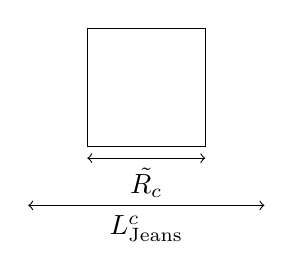
\begin{tikzpicture}[scale=1.5]
			\draw (0, 0) -- (1, 0) -- (1, 1) -- (0, 1) -- (0, 0);
			\draw[<->] (0, -0.1) -- (1, -0.1);
			\draw (0.5, -0.1) node[below] {$\tilde{R_c}$};
			\draw[<->] (-0.5, -0.5) -- (1.5, -0.5);
			\draw (0.5, -0.5) node[below] {$L_\mathrm{Jeans}^c$};
		\end{tikzpicture}
	\end{wrapfigure}
	Vouloir faire une simulation avec un cube interagissant, c'est bien beau, mais un tel objet risque de s'effondrer plutôt vite. Il va nous falloir une condition pour pouvoir le stabiliser.
	Une sphère homogène est stable si sa taille est inférieur à sa longueur de Jeans. Notre critère est donc le suivant:
	\begin{align}
		\tilde{R_c} &< L_\mathrm{Jeans}^c = \frac{\sigma_c}{\sqrt{GM_c}} \notag \\
		\tilde{R_c}^2 &< \frac{\sigma_c^2}{GM_c} \notag \\
		GM_c\tilde{R_c}^2 &< \sigma_c^2
	\end{align}
	Nous imposons aux particules du cube d'avoir la même masse que celle du Hénon, soit:
	\begin{align*}
		m_c = m_h = \dfrac{M_h}{N_h}
	\end{align*}
	où $N_h$ est le nombre de particules du Hénon. Soit $N_c$ le nombre de particules du cube,
	notre critère devient:
	\begin{align}
		GM_h\dfrac{N_c}{N_h}\tilde{R_c}^2 &< \sigma_c^2 \notag \\
		\dfrac{N_c}{N_h}\tilde{R_c}^2 &< \sigma_c^2 \notag \\
		\dfrac{N_c}{N_h} &< \dfrac{\sigma_c^2}{\tilde{R_c}^2} \label{simu::eq::idee4_jeans}
	\end{align}
	en oubliant pas que: $G=1$ et $M_h=1$.

\subsection{Conditions de la simulation}
	Comme nous cherchons à vérifier notre modèle, nous devons placer le bain à une température
	inférieur à celle que la sphère de Hénon atteint une fois à l'équilibre. Soit $\sigma_h^f$ la
	dispersion de vitesse de la sphère après effondrement, on doit avoir:
	\begin{align}
		\sigma_c &< \sigma_h^f \label{simu::eq::idee4_sig}
	\end{align}

	En parallèle, il serait bon d'éviter que le bain détruise la sphère de Hénon. Il faudrait
	donc imposer:
	\begin{align}
		\rho_\mathrm{bord}^f \geq \rho_c \label{simu::eq::idee4_dens}
	\end{align}
	où $\rho_\mathrm{bord}^f$ représente la densité au bord de la sphère, une fois l'équilibre
	atteint.

\subsection{critères de sélections des paramètres}
	En combinant les équations \ref{simu::eq::idee4_dens}, \ref{simu::eq::idee4_sig} et
	\ref{simu::eq::idee4_jeans}, nous obtenons l'ensemble d'équations suivant:
	\begin{align}
		\begin{cases}
			\(\frac{4}{3}\pi R_h^3\frac{N_c}{N_h}\)^{1/3} < R_c \\
			\\
			\(\frac{N_c}{N_h}\)^{5/3} R_h^2 \(\frac{4}{3}\pi\)^{2/3} < \sigma_c^2 < \(\sigma_h^f\)^2
		\end{cases}
	\end{align}
	avec $R_h$ le rayon de la sphère une fois l'équilibre atteint, sans le bain.

